\documentclass{article}
\author{Sabrina et al... more al than Sabrina}
\usepackage{float}  % for [H] placement if needed
\usepackage{amsmath}
\usepackage{amssymb}
\usepackage{graphicx}
\usepackage{caption}
\usepackage{amsmath, amssymb, bm}

\title{Generalizing GLV to Autotoxicity Model}
\date{February 2025}
\begin{document}

\maketitle

\section{Generalizing GLV to Autotoxicity Model}

Our starting point is the GLV:
\begin{equation}
\dot{n}_i = n_i\left( r_i - C_{ii} n_i - \sum_{j(\neq i)} C_{ij} n_j \right)
\end{equation}
This is a phenomenological and not a mechanistic model. The intra-specific suppression term, for instance, is meant to roughly capture the net effect of a variety of processes: conspecifics competition over resources, space, the effect of pathogens -- and autotoxicity. 

We should therefore think of the autotoxicity model as \emph{unpacking} some of the biological processes hidden in the phenomenological self-suppression term, rather than adding new mechanisms \emph{on top} of what's already represented by the GLV. This gives the generalization:
\begin{equation}
\dot{n}_i = n_i\left( r - C_{ii} h(n_i,a_i) - \sum_{j(\neq i)} C_{ij} n_j \right),
\end{equation}
with $a_i$ the autotoxin concentration. We want to preserve, in a sense, the interpretation of $C_{ii}$ as the net strength of self-suppression effects. The function $h(n,a)$ should partition these effects into a fraction $\gamma$ due to autotoxicity and the remaining fraction $1-\gamma$ due to the other implicit causes.

If we assume that individuals die due to autotoxicity at a rate proportional to the autotoxin concentration, then $h(n,a)$ is linear in both arguments. To have a notion of partitioning between $a$ and $n$, we must find what amount of $n$ constitutes an "equivalent" amount of $a$.

To this end, consider the autotoxicity dynamics. Production occurs at a per capita rate $\beta$ and degradation/dilution at a rate $\delta$:
\begin{equation}
\dot{a}_i = \beta n_i - \delta a_i.
\end{equation}
The formal solution is:
\begin{equation}
a_i(t) = \frac{\beta}{\delta} \int_{-\infty}^t K_\delta(t-s) n_i(s)\, ds
\end{equation}
where $K_\delta$ is an exponentially decaying memory kernel:
\begin{equation}
K_\delta(s) = \delta e^{-\delta|s|} \quad \Rightarrow \quad \int_{-\infty}^0 K_\delta(s)\, ds = 1
\end{equation}
We can therefore write:
\begin{equation}
a_i(t) = \frac{\beta}{\delta}\hat{n}_i(t)
\end{equation}b
where $\hat{n}_i$ is a historical weighted average of the abundance. The ratio $\beta/\delta$ is therefore the "conversion ratio" between suppression from autotoxicity and implicit density-dependent effects. The "unpacking" due to autotoxicity can be interpreted as:
\begin{equation}
C_{ii}n_i \rightarrow C_{ii}\left[ \gamma \hat{n}_i + (1-\gamma)n_i \right].
\end{equation}
Writing out the abundance dynamics in full:
\begin{equation}
\dot{n}_i = n_i\left[ r - C_{ii} \left(\gamma \frac{\delta}{\beta}a_i + (1-\gamma)n_i\right) - \sum_{j(\neq i)} C_{ij} n_j \right]
\end{equation}
There are \emph{three ways} that the autotoxicity model can exactly reduce to the GLV in this representation:
\begin{itemize}
  \item $\gamma \to 0$ (trivially)
  \item $\delta \to \infty$ (so that $\hat{n}_i \to n_i$)
  \item $\delta \to 0$ (but this is meaningless because autotoxicities explode)
\end{itemize}
For any values of $\gamma,\delta,\beta$, the fixed points are identical to those of the original GLV, although the stability properties can differ; the Jacobian of the autotoxicity model depends separately on these three parameters (compare Onofrio's notes).

\subsection{Comparison to Previous Parametrization}
Before we had written the model as:
\begin{equation}
\dot{n}_i / n_i = g ( 1 - \rho a_i ) - \sum_{j} B_{ij} n_j
\end{equation}
with the diagonal elements sometimes $B_{ii}=1$ other times $B_{ii}=0$, causing some confusion. Comparing the versions we have:
\begin{equation}
r=g, \quad C_{ii} \gamma \delta/\beta = g \rho, \quad C_{ii}(1-\gamma) = B_{ii}
\end{equation}

\subsection{Nondimensionalization}
To simplify the study of the model, we make use of the fact that the arbitrary choice of units to measure time, abundance, and autotoxicity concentration allow us to reduce the number of relevant parameters by three. A detailed analysis proceeds by substituting:
\begin{equation}
n = N\tilde{n}, \quad a = A\tilde{a}, \quad t= T\tilde{t}
\end{equation}
in the dynamics, where the tilde-variable is nondimensional and the capital letter is the units of measurement to be decided. This leads one to conclude that the natural choice is:
\begin{equation}
T = 1/r, \quad N= r/C_{ii}, \quad A=\beta/C_{ii}.
\end{equation}
Note that this only works if $C_{ii}$ does not depend on $i$, but this we assume. We similarly nondimensionalise the other parameters:
\begin{equation}
\beta = \tilde{\beta}A/TN, \quad \delta = \tilde{\delta}/T, \quad C_{ij} = \tilde{C}_{ij}TN.
\end{equation}
In practice, this procedure is equivalent to simply putting $r=1,\beta=1,C_{ii}=1$ and dropping all the tildes. Thus, the simplified model is:
\begin{align}
\dot{n}_i &= n_i\left[ 1 - \left(\gamma \delta a_i + (1-\gamma)n_i\right) - \sum_{j(\neq i)} C_{ij} n_j \right] \\
\dot{a}_i &= n_i - \delta a_i
\end{align}
We draw $C_{ij}\sim \mathcal{N}(\mu,\sigma)$, i.e., not with weak interaction scaling. In the end there are (beside species richness $S$) four continuous parameters to study: $\mu,\sigma,\delta,\gamma$.

\subsection{Agenda}
To understand how the $(\mu,\sigma)$ phase diagram of the GLV (not assuming weak scaling) is extended in the $\delta,\gamma$ directions.
\begin{enumerate}
    \item First look at dynamics versus $\delta,\gamma$ for few pairs $(\mu,\sigma)$ lying in the different phases in the GLV case
    \item Assuming we then find a fixed $\delta$ for which $\gamma$ can change stability, do numerical bifurcation diagram in $\gamma$ to determine type. (Perhaps complement with Jacobian spectrum plots)
    \item For the GLV, an arc in $(\mu,\sigma)$-space with not-too-large radius $\mu_0$ and focal point $(1,0)$ will cross all the boundaries of non-diverging phases perpendicularly. With $\phi$ the angle of such an arc, look at the dynamics in the $(\phi,\gamma)$-plane for some fixed $\delta$, or in $(\phi,\delta)$-plane for $\gamma=1$.
\end{enumerate}

We move forward after getting a sense of the range of the dynamics from these studies.



\title{Simulation Results}
\author{}
\date{May 2025}
\maketitle
\section{Single species dynamics: S=1}
\begin{align}
\dot{n} &= n\left( 1 - \gamma \delta a - (1 - \gamma)n \right),\\
\dot{a} &= n - \delta a,\\
\end{align}
\subsection*{Eigenvalue Derivation for the Single-Species Autotoxicity Model}

We consider the system:
\begin{align}
\dot{n} &= n\left( 1 - \gamma \delta a - (1 - \gamma)n \right) \\
\dot{a} &= n - \delta a
\end{align}

\subsubsection*{Fixed Point}

At equilibrium, set $\dot{n} = 0$ and $\dot{a} = 0$:
\[
n = \delta a \quad \Rightarrow \quad a = \frac{n}{\delta}
\]
Substitute into the first equation:
\[
\dot{n} = n \left( 1 - \gamma a n - (1 - \gamma) n \right) = n(1 - n)
\Rightarrow n^* = 1, \quad a^* = \frac{1}{\delta}
\]


\begin{figure}[H]
    \centering
    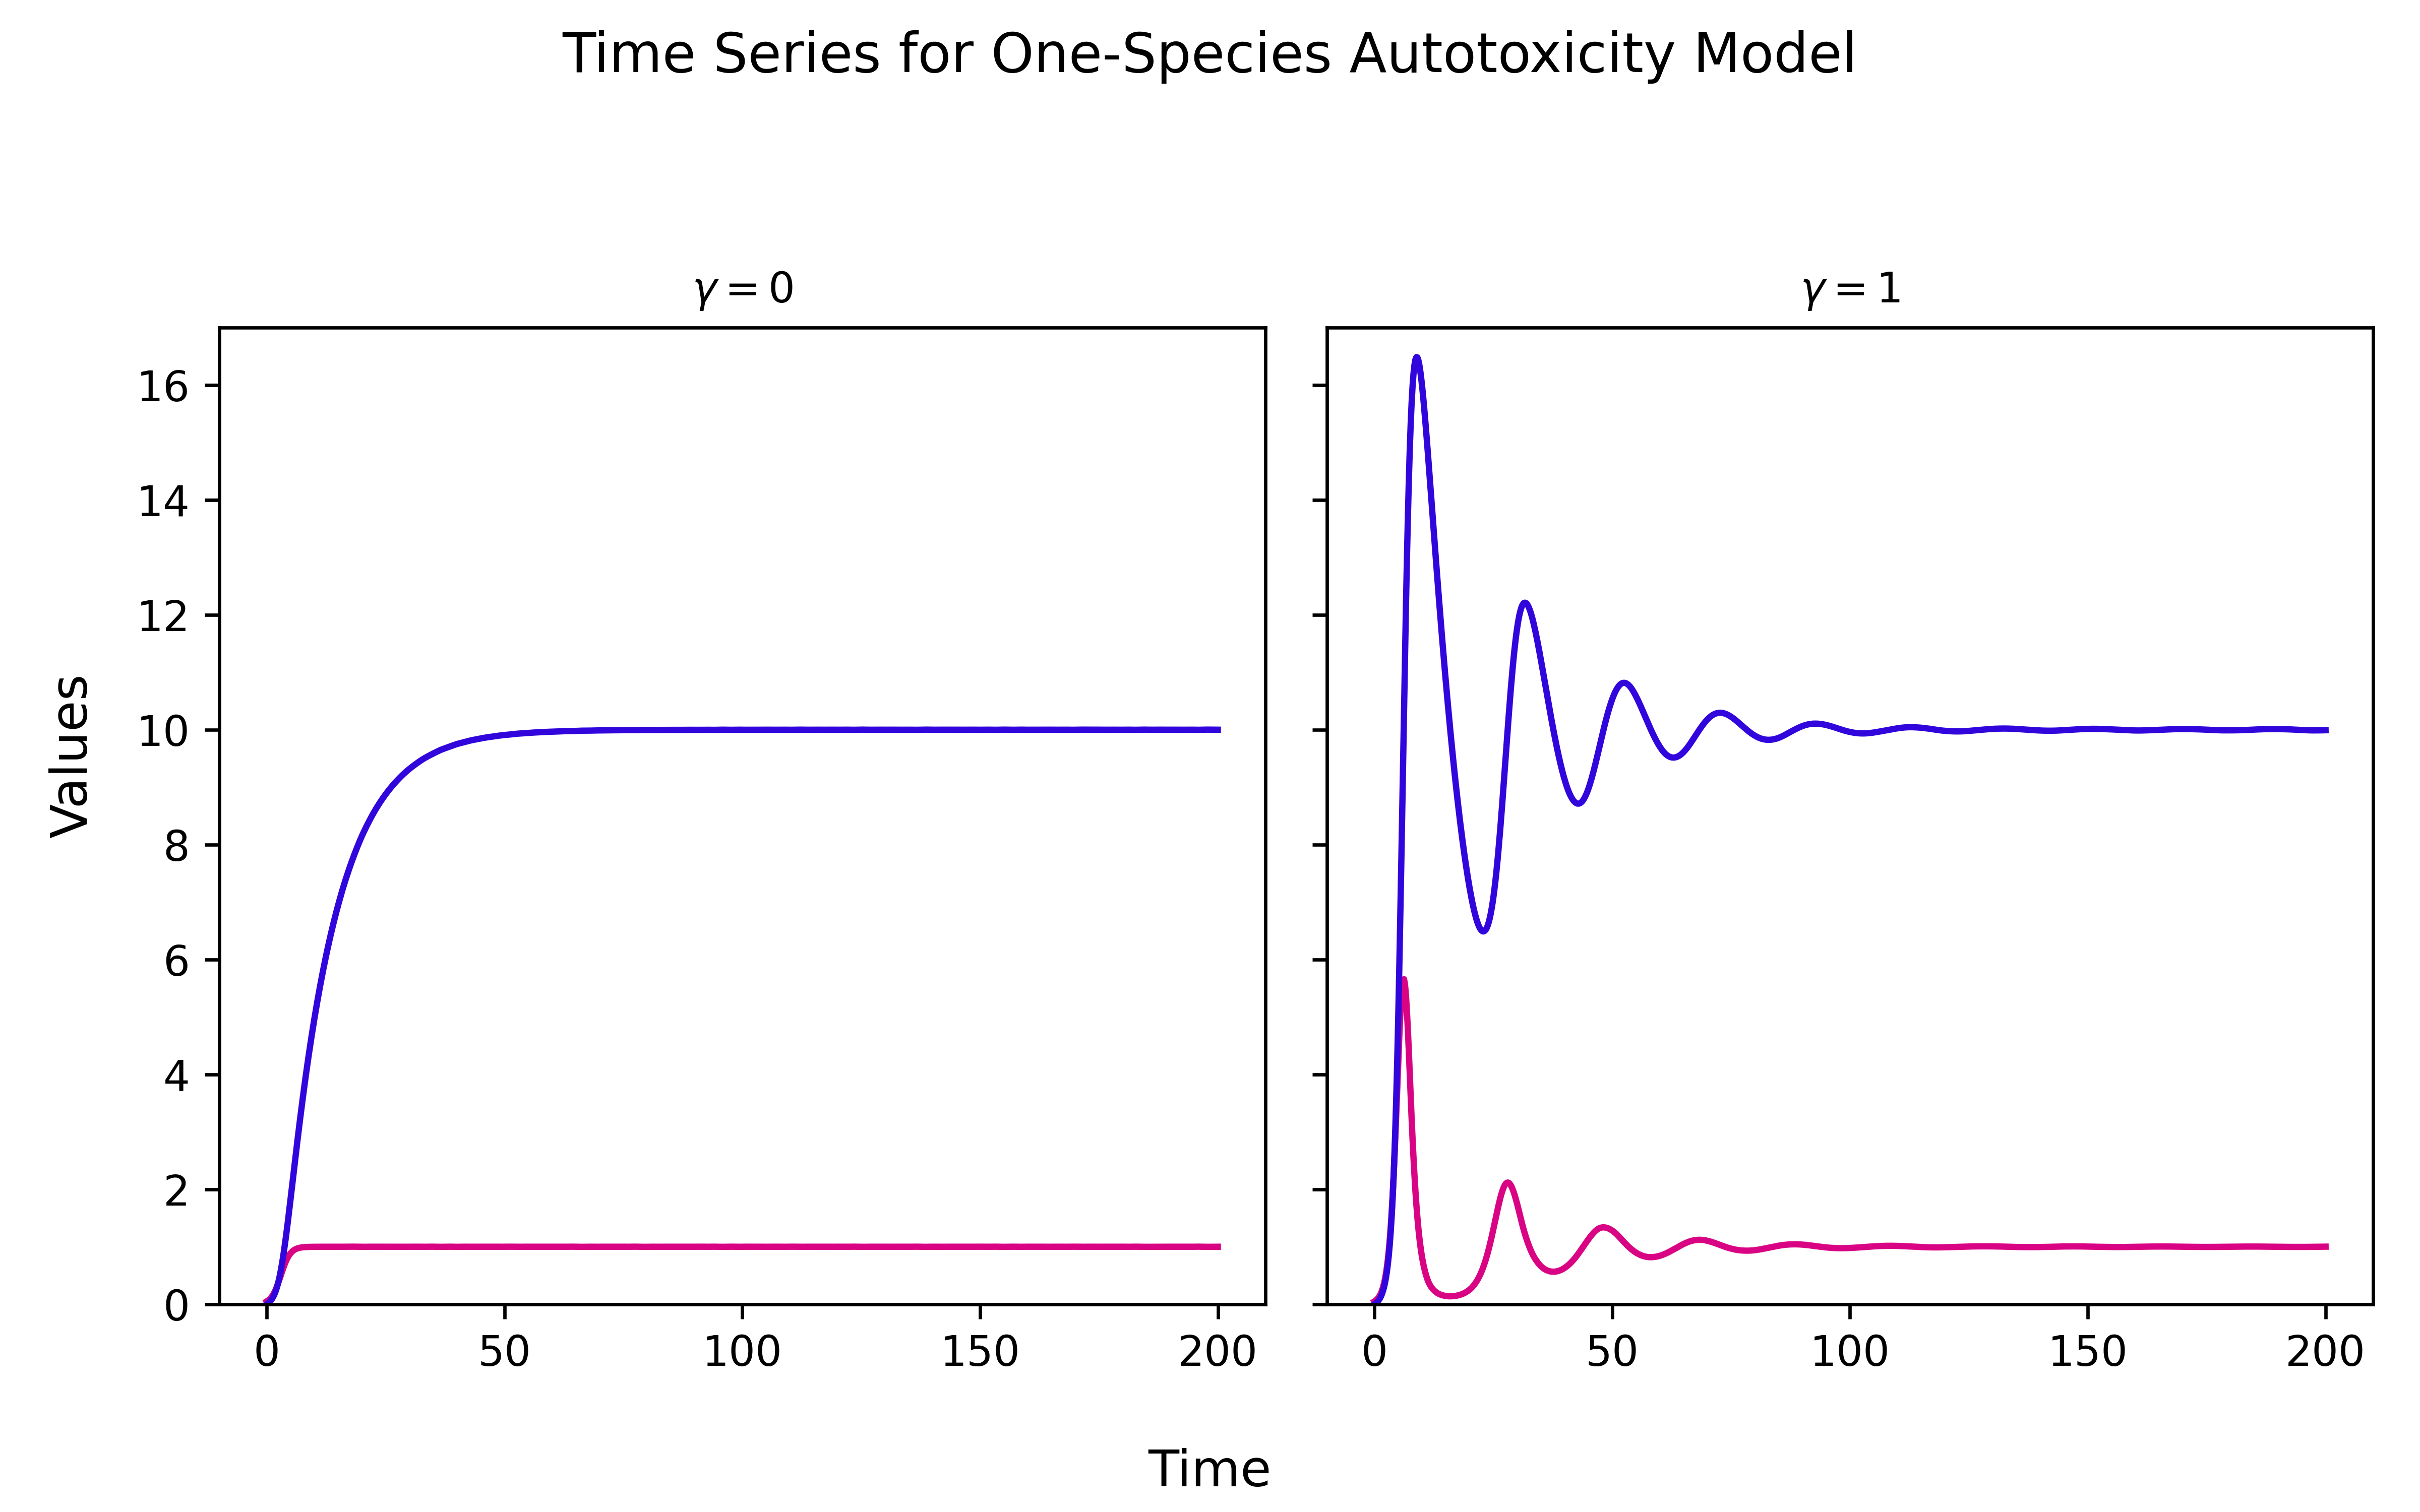
\includegraphics[width=\linewidth]{SingleSpecies/time_series_single_species.png}
    \caption{Species (Pink) and Autotoxicity (Purple) dynamics in Linear space with $\gamma$=0 on the left and $\gamma$=1 on the right.}
\end{figure}
\clearpage

\subsubsection*{Jacobian Matrix}

Define:
\[
f(n, a) = n \left( 1 - \gamma \delta a - (1 - \gamma)n \right), \quad 
g(n, a) = n - \delta a
\]

Compute the Jacobian $J$:
\[
J = 
\begin{pmatrix}
J_{nn} & J_{na} \\
J_{an} & J_{aa}
\end{pmatrix}
\]

At the fixed point $(n^*, a^*) = (1, 1/\delta)$:
\begin{align*}
J_{nn} &= 1 - \gamma \delta a - 2(1 - \gamma)n = -1 + \gamma \\
J_{na} &= -\gamma \delta \\
J_{an} &= 1\\
J_{aa}&= -\delta\\
\end{align*}

\[
J =
\begin{pmatrix}
-1 + \gamma & -\gamma \delta \\
1 & -\delta
\end{pmatrix}
\]
\clearpage
\subsubsection*{Characteristic Equation and Eigenvalues}

We compute the eigenvalues by solving:
\[
\det(J - \lambda I) = 0
\]

\[
\begin{vmatrix}
-1 + \gamma - \lambda & -\gamma \delta \\
1 & -\delta - \lambda
\end{vmatrix}
= 0
\]

\[
(-1 + \gamma - \lambda)(-\delta - \lambda) + \gamma \delta = 0
\]

\[
(\lambda + 1 - \gamma)(\lambda + \delta) + \gamma \delta = 0
\]

\[
\lambda^2 + (1 - \gamma + \delta)\lambda + (1 - \gamma)\delta + \gamma \delta = 0
\]

\[
\lambda^2 + \left( (1 - \gamma) + \delta \right)\lambda + \delta = 0
\]

\subsubsection*{Eigenvalue Formula}

The eigenvalues are:
\[
\lambda = -\frac{(1 - \gamma) + \delta}{2} 
\pm 
\sqrt{\left( \frac{(1 - \gamma) + \delta}{2} \right)^2 - \delta}
\]

\begin{figure}[H]
    \centering
    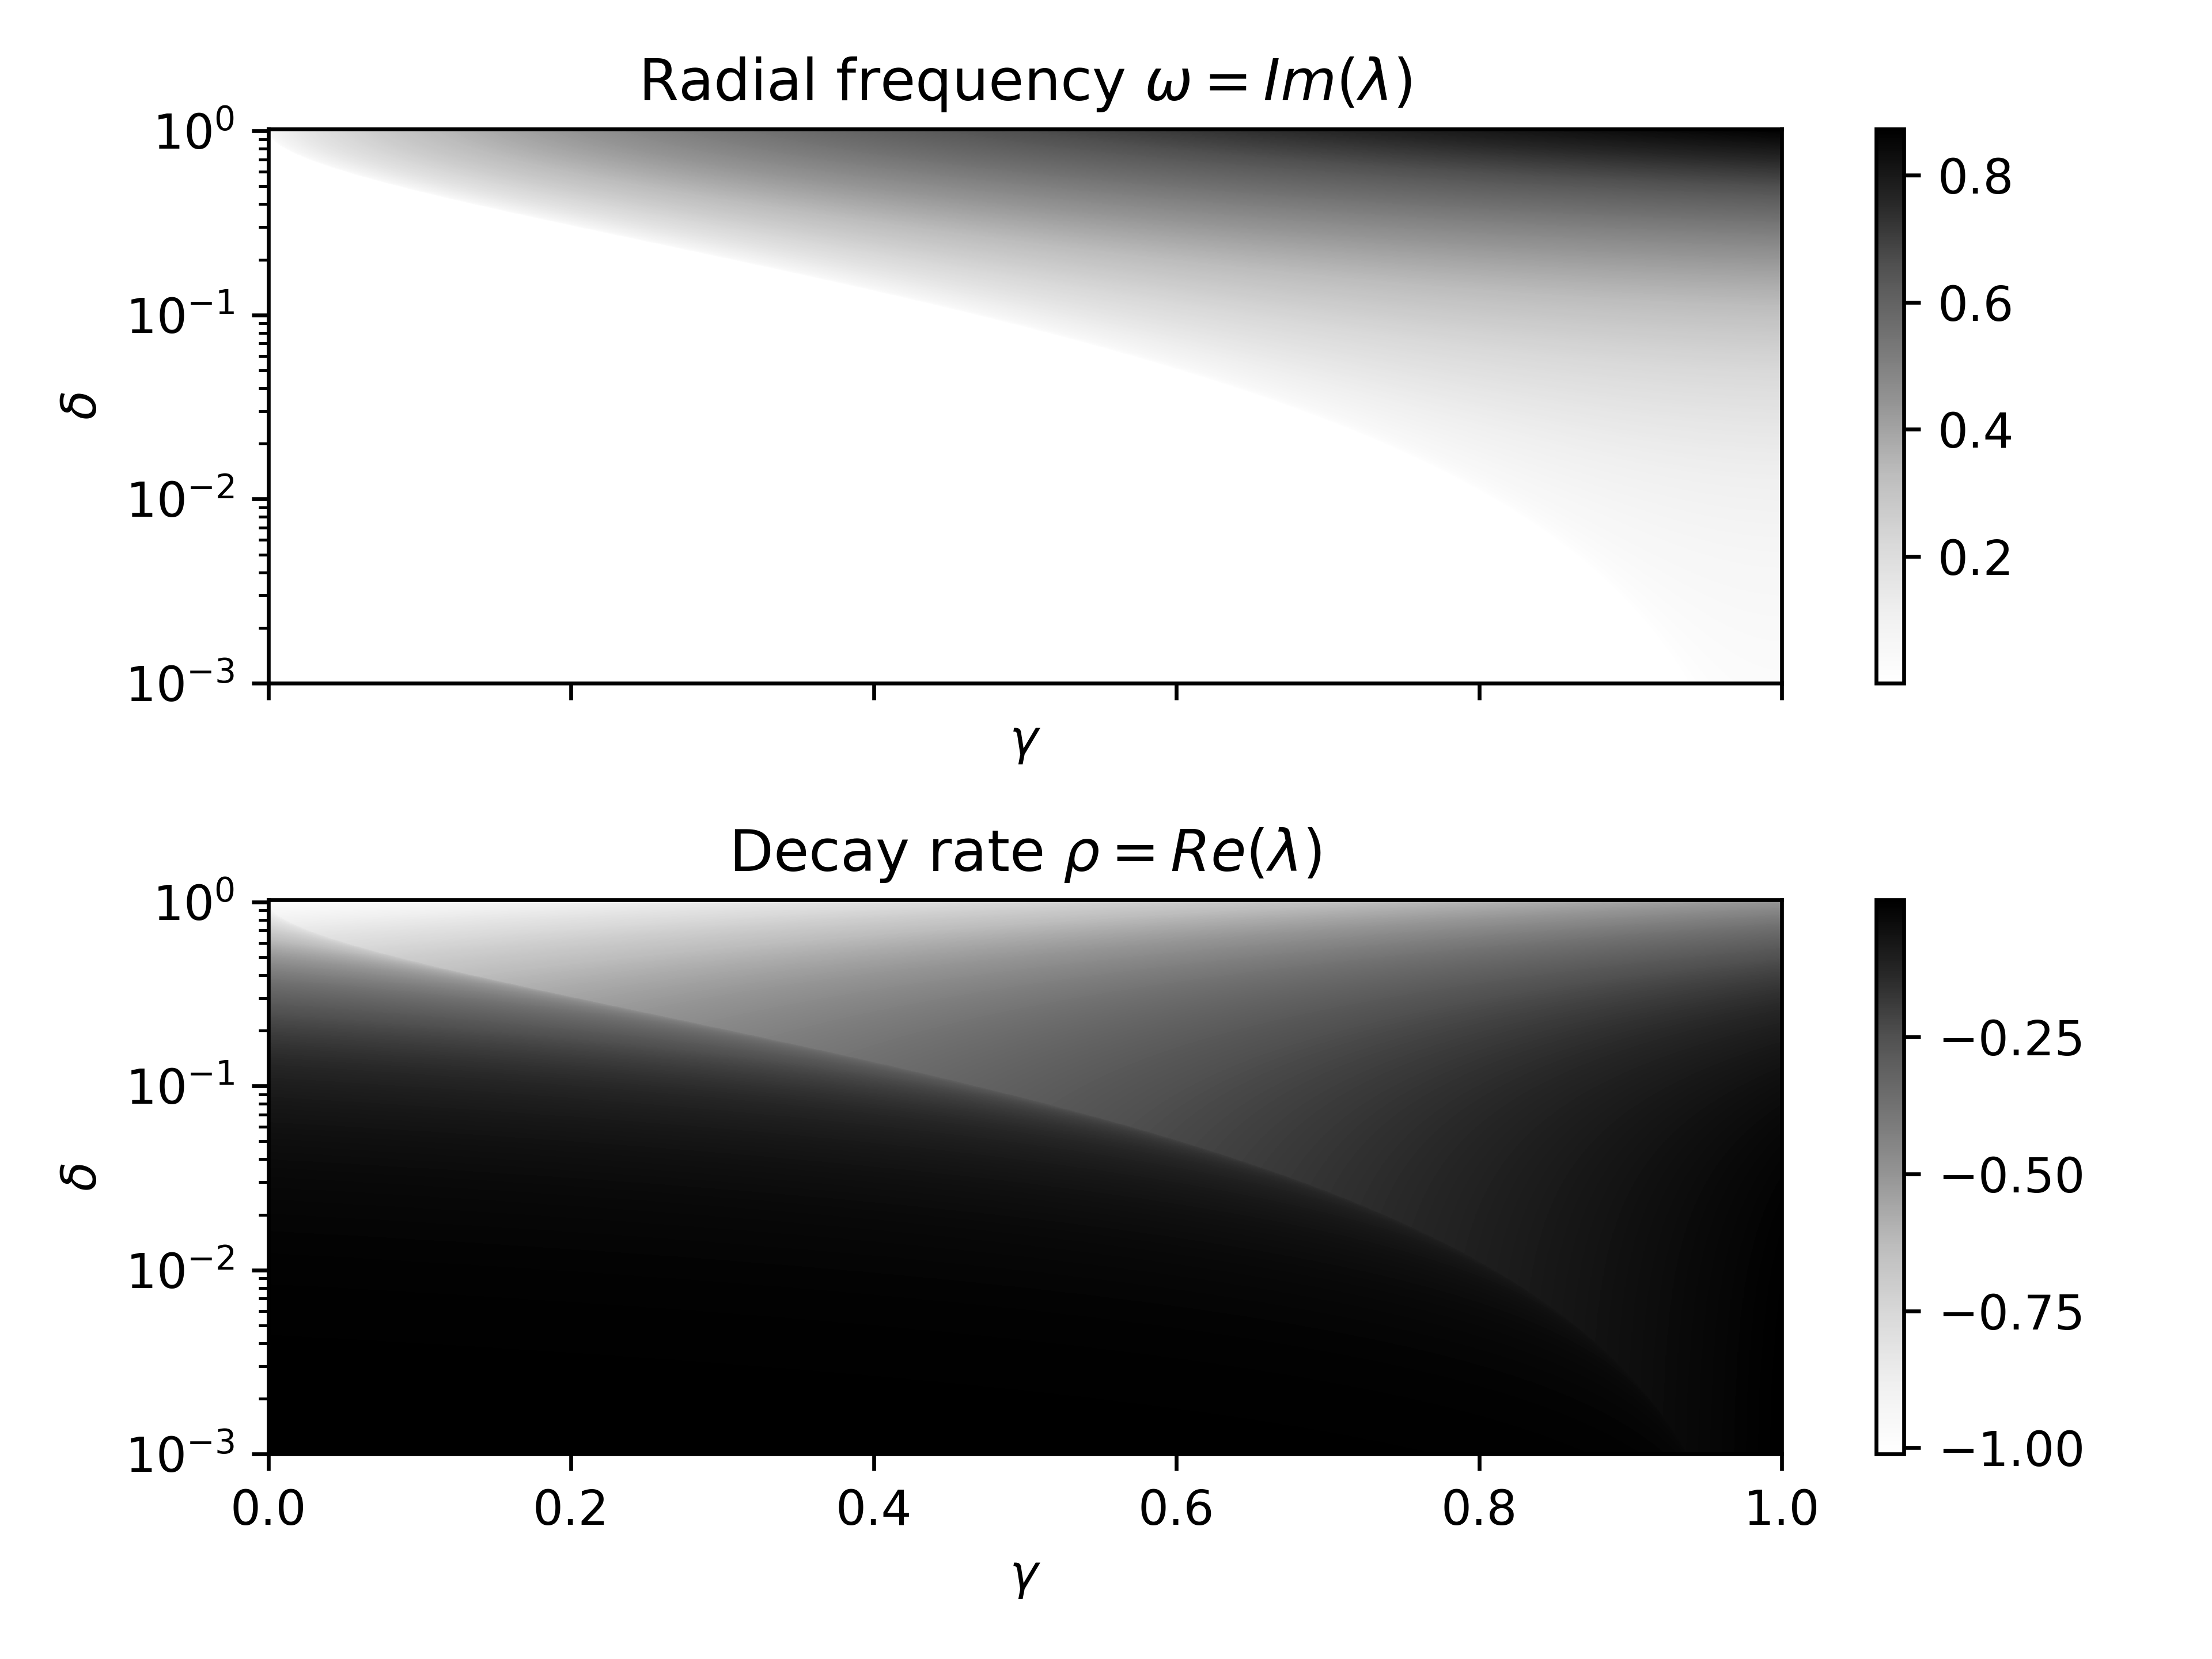
\includegraphics[width=\linewidth]{SingleSpecies/RadFreq.png}
    \caption{Imaginary and real parts of the eigenvalues as a function of $\gamma$ and $\delta$.}
    \label{fig:RealandImaginaryPart}
\end{figure}


\paragraph{Figure~\ref{fig:RealandImaginaryPart} shows a heatmap of the real and imaginary parts of the eigenvalues for different values of $\delta$ and $\gamma$.
How to interpret:}
\begin{itemize}
    \item The \textbf{real part} $\text{Re}(\lambda)$ determines the decay rate or growth.
        \begin{itemize}
            \item If $\text{Re}(\lambda) < 0$, the system decays to equilibrium (stable).
            \item If $\text{Re}(\lambda) > 0$, the system is unstable.
        \end{itemize}
    \item The \textbf{radial frequency} $\omega = \text{Im}(\lambda)$ determines the frequency of oscillation (ignoring decay).
        \begin{itemize}
            \item If $\omega = 0$, no oscillation.
            \item If $0 < \omega < 1$, the oscillations are slow.
        \end{itemize}
In the current system, the decay rate is always negative, meaning the system is stable. The radial frequency remains below 1, indicating slow oscillations. Taken together, this implies that the system exhibits \textbf{damped oscillations} — it spirals into the fixed point.
\end{itemize}

\clearpage

\section{Two Species Dynamics: $S=2$}


\begin{figure}[H]
    \centering

    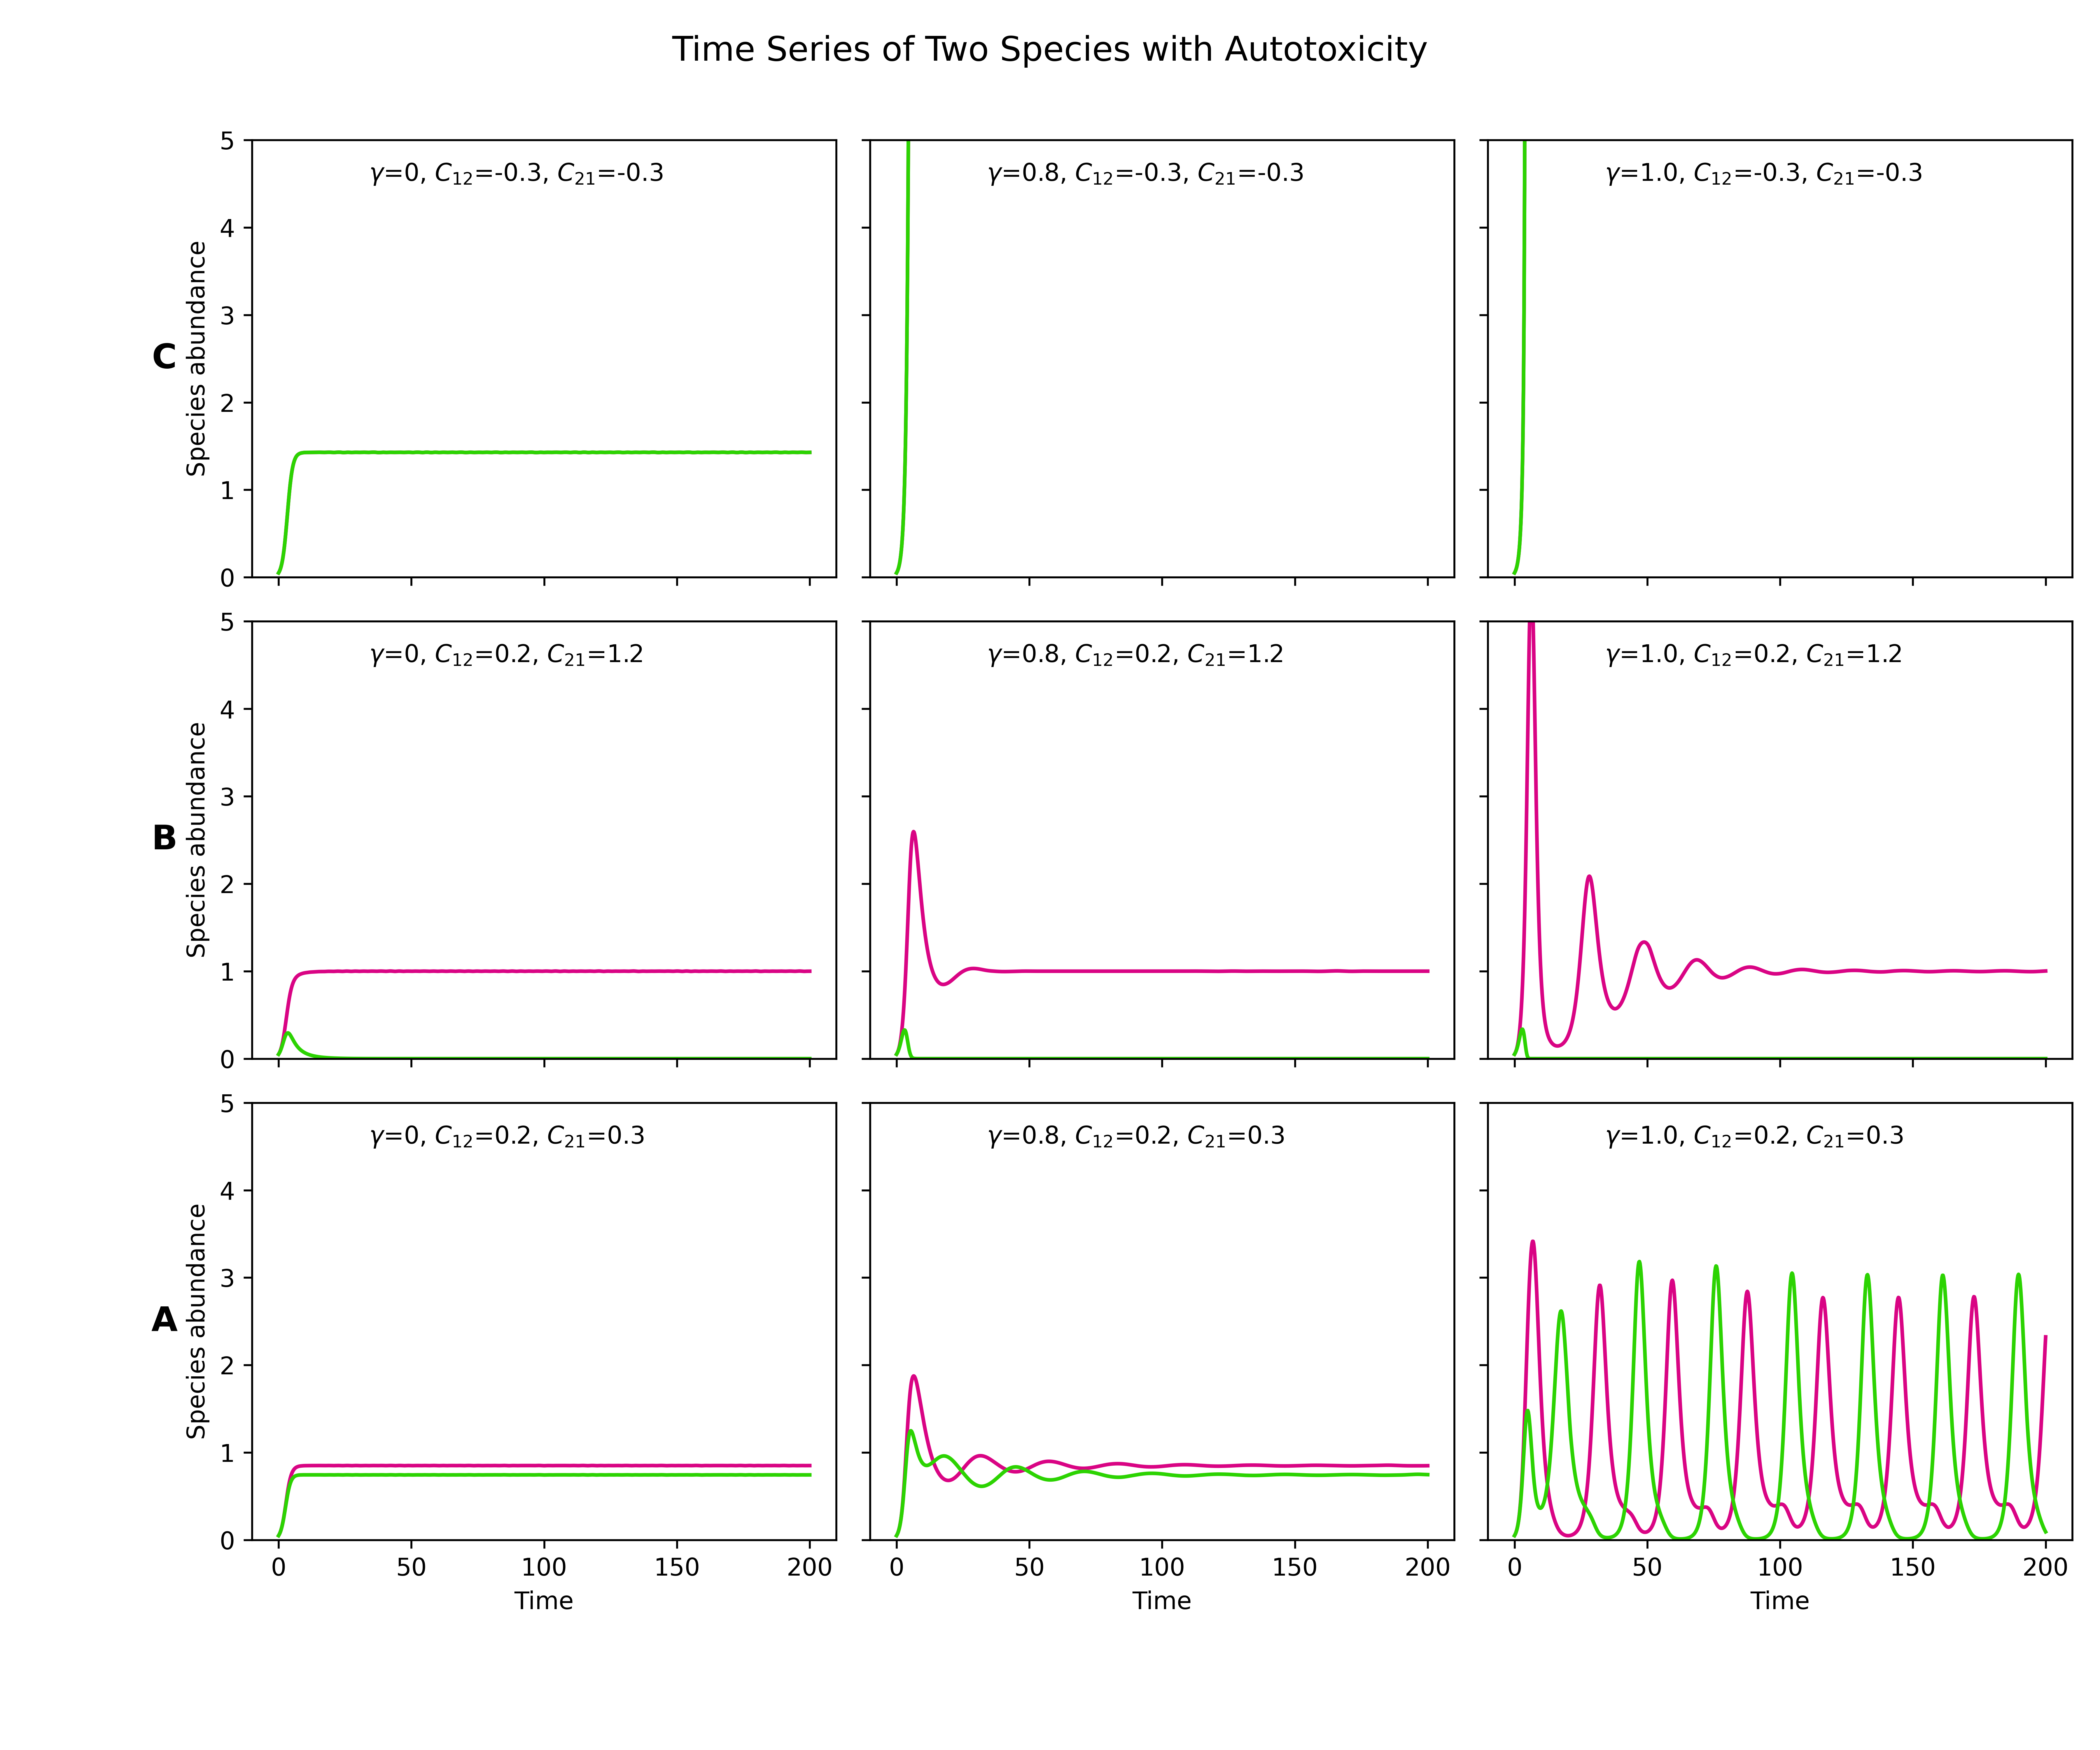
\includegraphics[width=\linewidth]{SingleSpecies/TwoSpecies3Cases.png}
    \caption{Species 1 (green) and Species 2 (pink) dynamics in linear space with $\gamma=0$, $\gamma=0.8$, and $\gamma=1$. The interaction between the two species varies from top to bottom. 
    (A) Both species positively influence each other with equal interaction strengths. 
    (B) The species compete, and Species 2 exerts a stronger negative influence on Species 1. 
    (C) The species compete, with Species 2 having a slightly higher competition parameter.}
    \label{fig:twospecies}
\end{figure}

The dynamics of two species is showed in Figure~\ref{fig:twospecies}, with 3 different values of $\gamma$ and 3 different combinations of $C_{12}$ and $C_{21}$.
When $C_{12}$ and $C_{21}$ are both negative (meaning that they cooperate) --first row of the panel--, the increasing of autotoxicity-- from the left to the side-- lead the system to explode. Looking at the second row of the panel, when the species compete, -- and species 2 has an higher competitive parameter $C_{21}$=1.2, the species will not cohexist and the increasing of autotoxicity will lead to the same result of the gLV. When the specie compete to each other with lower parameters of competition, increasing autotoxicity will lead to an "oscillatory" cohexistence between the two species. 
\begin{align}
\dot{n}_1 &= n_1 \left[ 1 - \left( \gamma \delta a_1 + (1 - \gamma) n_1 \right) - C_{12} n_2(t) \right] \tag{Species 1} \\
\dot{n}_2 &= n_2\left[ 1 - \left( \gamma \delta a_2 + (1 - \gamma) n_2 \right) - C_{21} n_1(t) \right] \tag{Species 2} \\
\dot{a}_1 &= n_1 - \delta a_1(t) \tag{Autotoxin 1} \\
\dot{a}_2 &= n_2 - \delta a_2(t) \tag{Autotoxin 2}
\end{align}




\clearpage

\section{Community dynamics: S=500}
We consider the log-transformed system of $S$ interacting species with autotoxicity. Let
\[
\bm{s} = 
\begin{bmatrix}
\log \bm{n} \\
\log \bm{a}
\end{bmatrix}
\in \mathbb{R}^{2S},
\]
where $\bm{n}, \bm{a} \in \mathbb{R}^S$ are the abundances and autotoxicity of each species.

The system is governed by the equations:
\begin{align*}
\frac{d}{dt} \log n_i &= 1 - \left( \gamma \delta a_i + (1 - \gamma) n_i \right) - \sum_{j \ne i} C_{ij} n_j + \frac{\lambda}{n_i}, \\
\frac{d}{dt} \log a_i &= \frac{n_i}{a_i} - \delta,
\end{align*}
with $n_i = e^{\log n_i}$ and $a_i = e^{\log a_i}$.

\subsection{Jacobian Analysis in log space}

We consider again the log-transformed system of $S$ interacting species with autotoxicity, with the equations:
\begin{align}
\frac{d}{dt} \log n_i &= 1 - \left( \gamma \delta a_i + (1 - \gamma) n_i \right) - \sum_{j \ne i} C_{ij} n_j + \frac{\lambda}{n_i}, \\
\frac{d}{dt} \log a_i &= \frac{n_i}{a_i} - \delta,
\end{align}
with $n_i = e^{\log n_i}$ and $a_i = e^{\log a_i}$.

\subsubsection{Equilibrium Condition}

At equilibrium:

\[
\begin{aligned}
1 - \gamma \delta a_i - (1 - \gamma) n_i - \sum_{j \ne i} C_{ij} n_j + \frac{\lambda}{n_i} &= 0, \\
\frac{n_i}{a_i} - \delta &= 0, \\
\text{Substitute into the first equation: } 
a_i &= \frac{n_i}{\delta}\\
1 - \gamma \delta \cdot \frac{n_i}{\delta} - (1 - \gamma) n_i - \sum_{j \ne i} C_{ij} n_j + \frac{\lambda}{n_i} &= 0, \\
- \sum_{j \ne i} C_{ij} n_j + \frac{\lambda}{n_i} &= 0 \\
\end{aligned}
\]
The equilibrium does depend on the interacting matrix but does not depend on $\gamma$ and $\delta$.
\subsubsection{Jacobian Matrix}

We define the Jacobian as:
\[
J =
\begin{bmatrix}
J_{nn} & J_{na} \\
J_{an} & J_{aa}
\end{bmatrix},
\]
where $\bm{f}(\bm{s}) = \frac{d\bm{s}}{dt}$.

\paragraph{Block $J_{nn}$:}
\[
\frac{\partial (\dot{\log n_i})}{\partial \log n_j} =
\begin{cases}
- C_{ij} \cdot n_j & \text{if } i \ne j, \\
- (1 - \gamma) n_i - \dfrac{\lambda}{n_i} & \text{if } i = j.
\end{cases}
\]

\paragraph{Block $J_{na}$:}
\[
\frac{\partial (\dot{\log n_i})}{\partial \log a_j} =
\begin{cases}
- \gamma \delta a_i & \text{if } i = j, \\
0 & \text{otherwise}.
\end{cases}
\]

\paragraph{Block $J_{an}$:}
\[
\frac{\partial (\dot{\log a_i})}{\partial \log n_j} =
\begin{cases}
\dfrac{n_i}{a_i} & \text{if } i = j, \\
0 & \text{otherwise}.
\end{cases}
\]

\paragraph{Block $J_{aa}$:}
\[
\frac{\partial (\dot{\log a_i})}{\partial \log a_j} =
\begin{cases}
- \dfrac{n_i}{a_i} & \text{if } i = j, \\
0 & \text{otherwise}.
\end{cases}
\]

\subsubsection{Stability Analysis}

The eigenvalues of $J$ determine local stability:
\[
\lambda_1, \dots, \lambda_{2S} = \texttt{eigvals}(J).
\]
\begin{itemize}
    \item If $\max \operatorname{Re}(\lambda_k) < 0$, the equilibrium is \textbf{locally stable}.
    \item If any $\operatorname{Re}(\lambda_k) > 0$, the system is \textbf{unstable}.
\end{itemize}
\clearpage

\subsection{Simulations $\sigma$–$\gamma$}
\[
C_{ij} \sim \mathcal{N}(\mu, \sigma), \quad 
\mu = 0.2,\quad \sigma \in [0.001, 0.1], \quad 
\gamma \in [0, 1], \quad \delta = 0.01, \quad \lambda = 10^{-8}
\]

\begin{figure}[H]
    \centering
    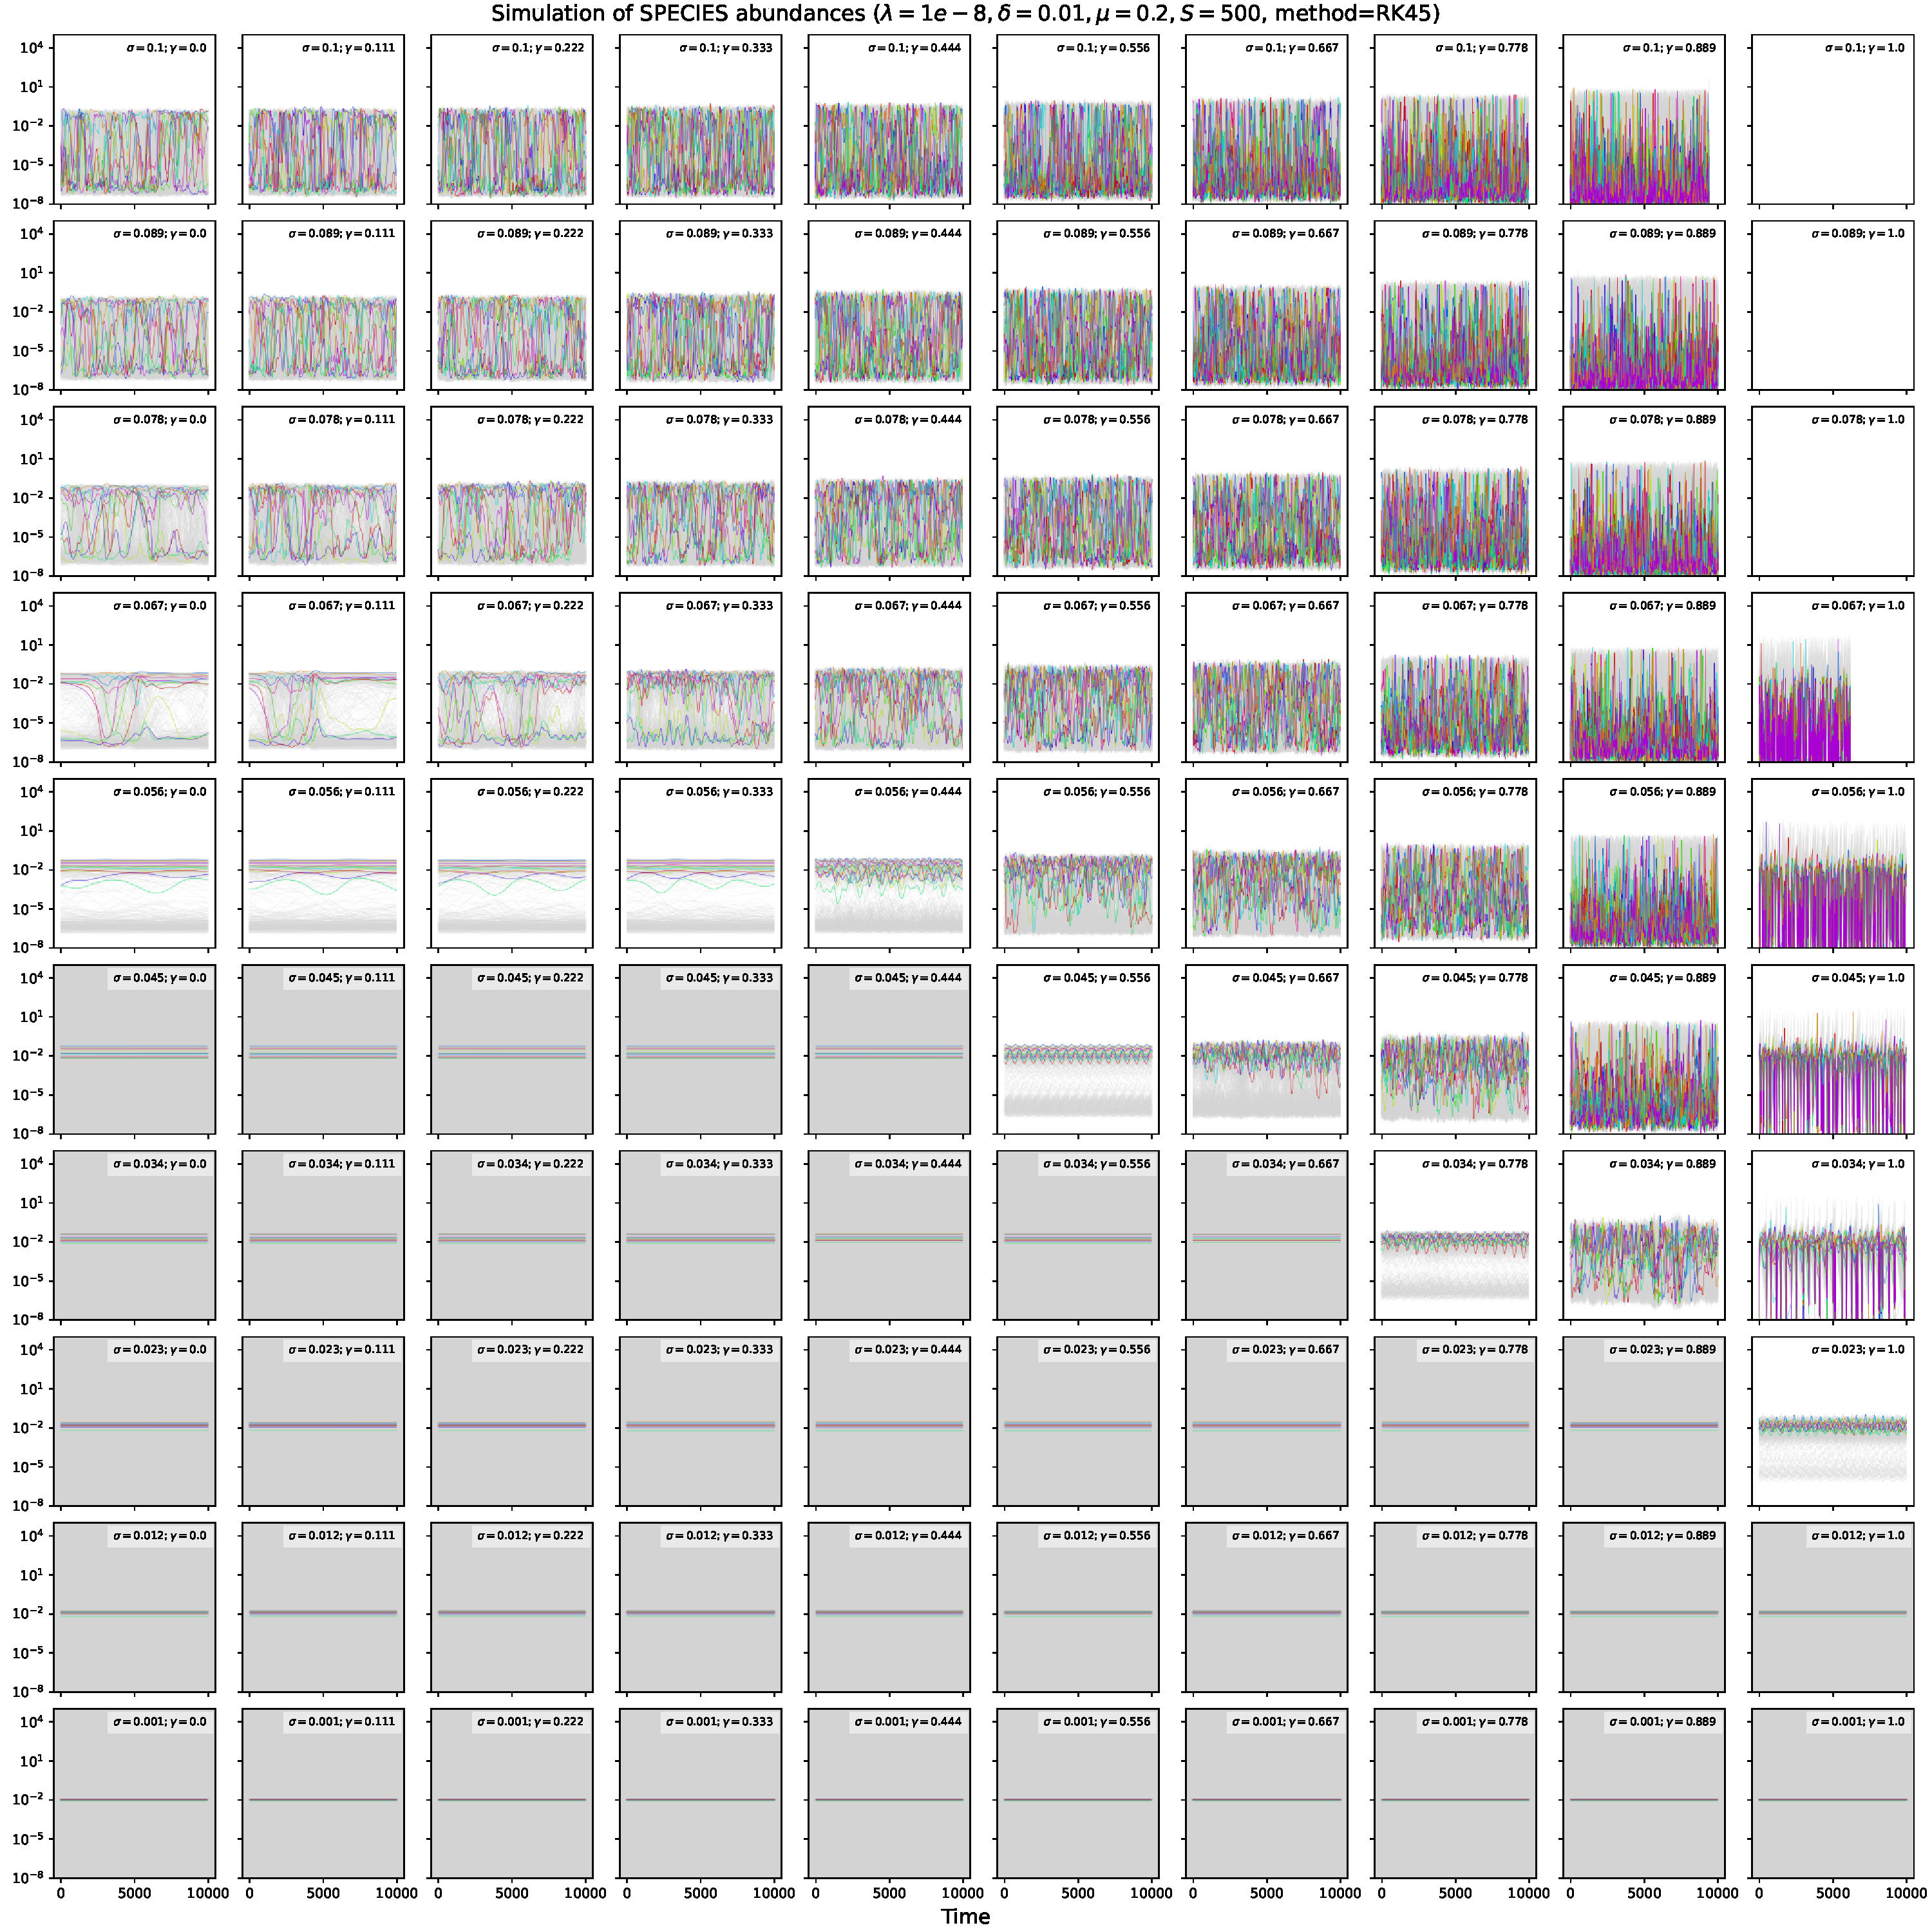
\includegraphics[width=\linewidth]{SigmaGamma/10Species.pdf}
    \caption{Species dynamics in logarithmic scale $\sigma$ and $\gamma$.}
\end{figure}

\clearpage

\begin{figure}[H]
    \centering
    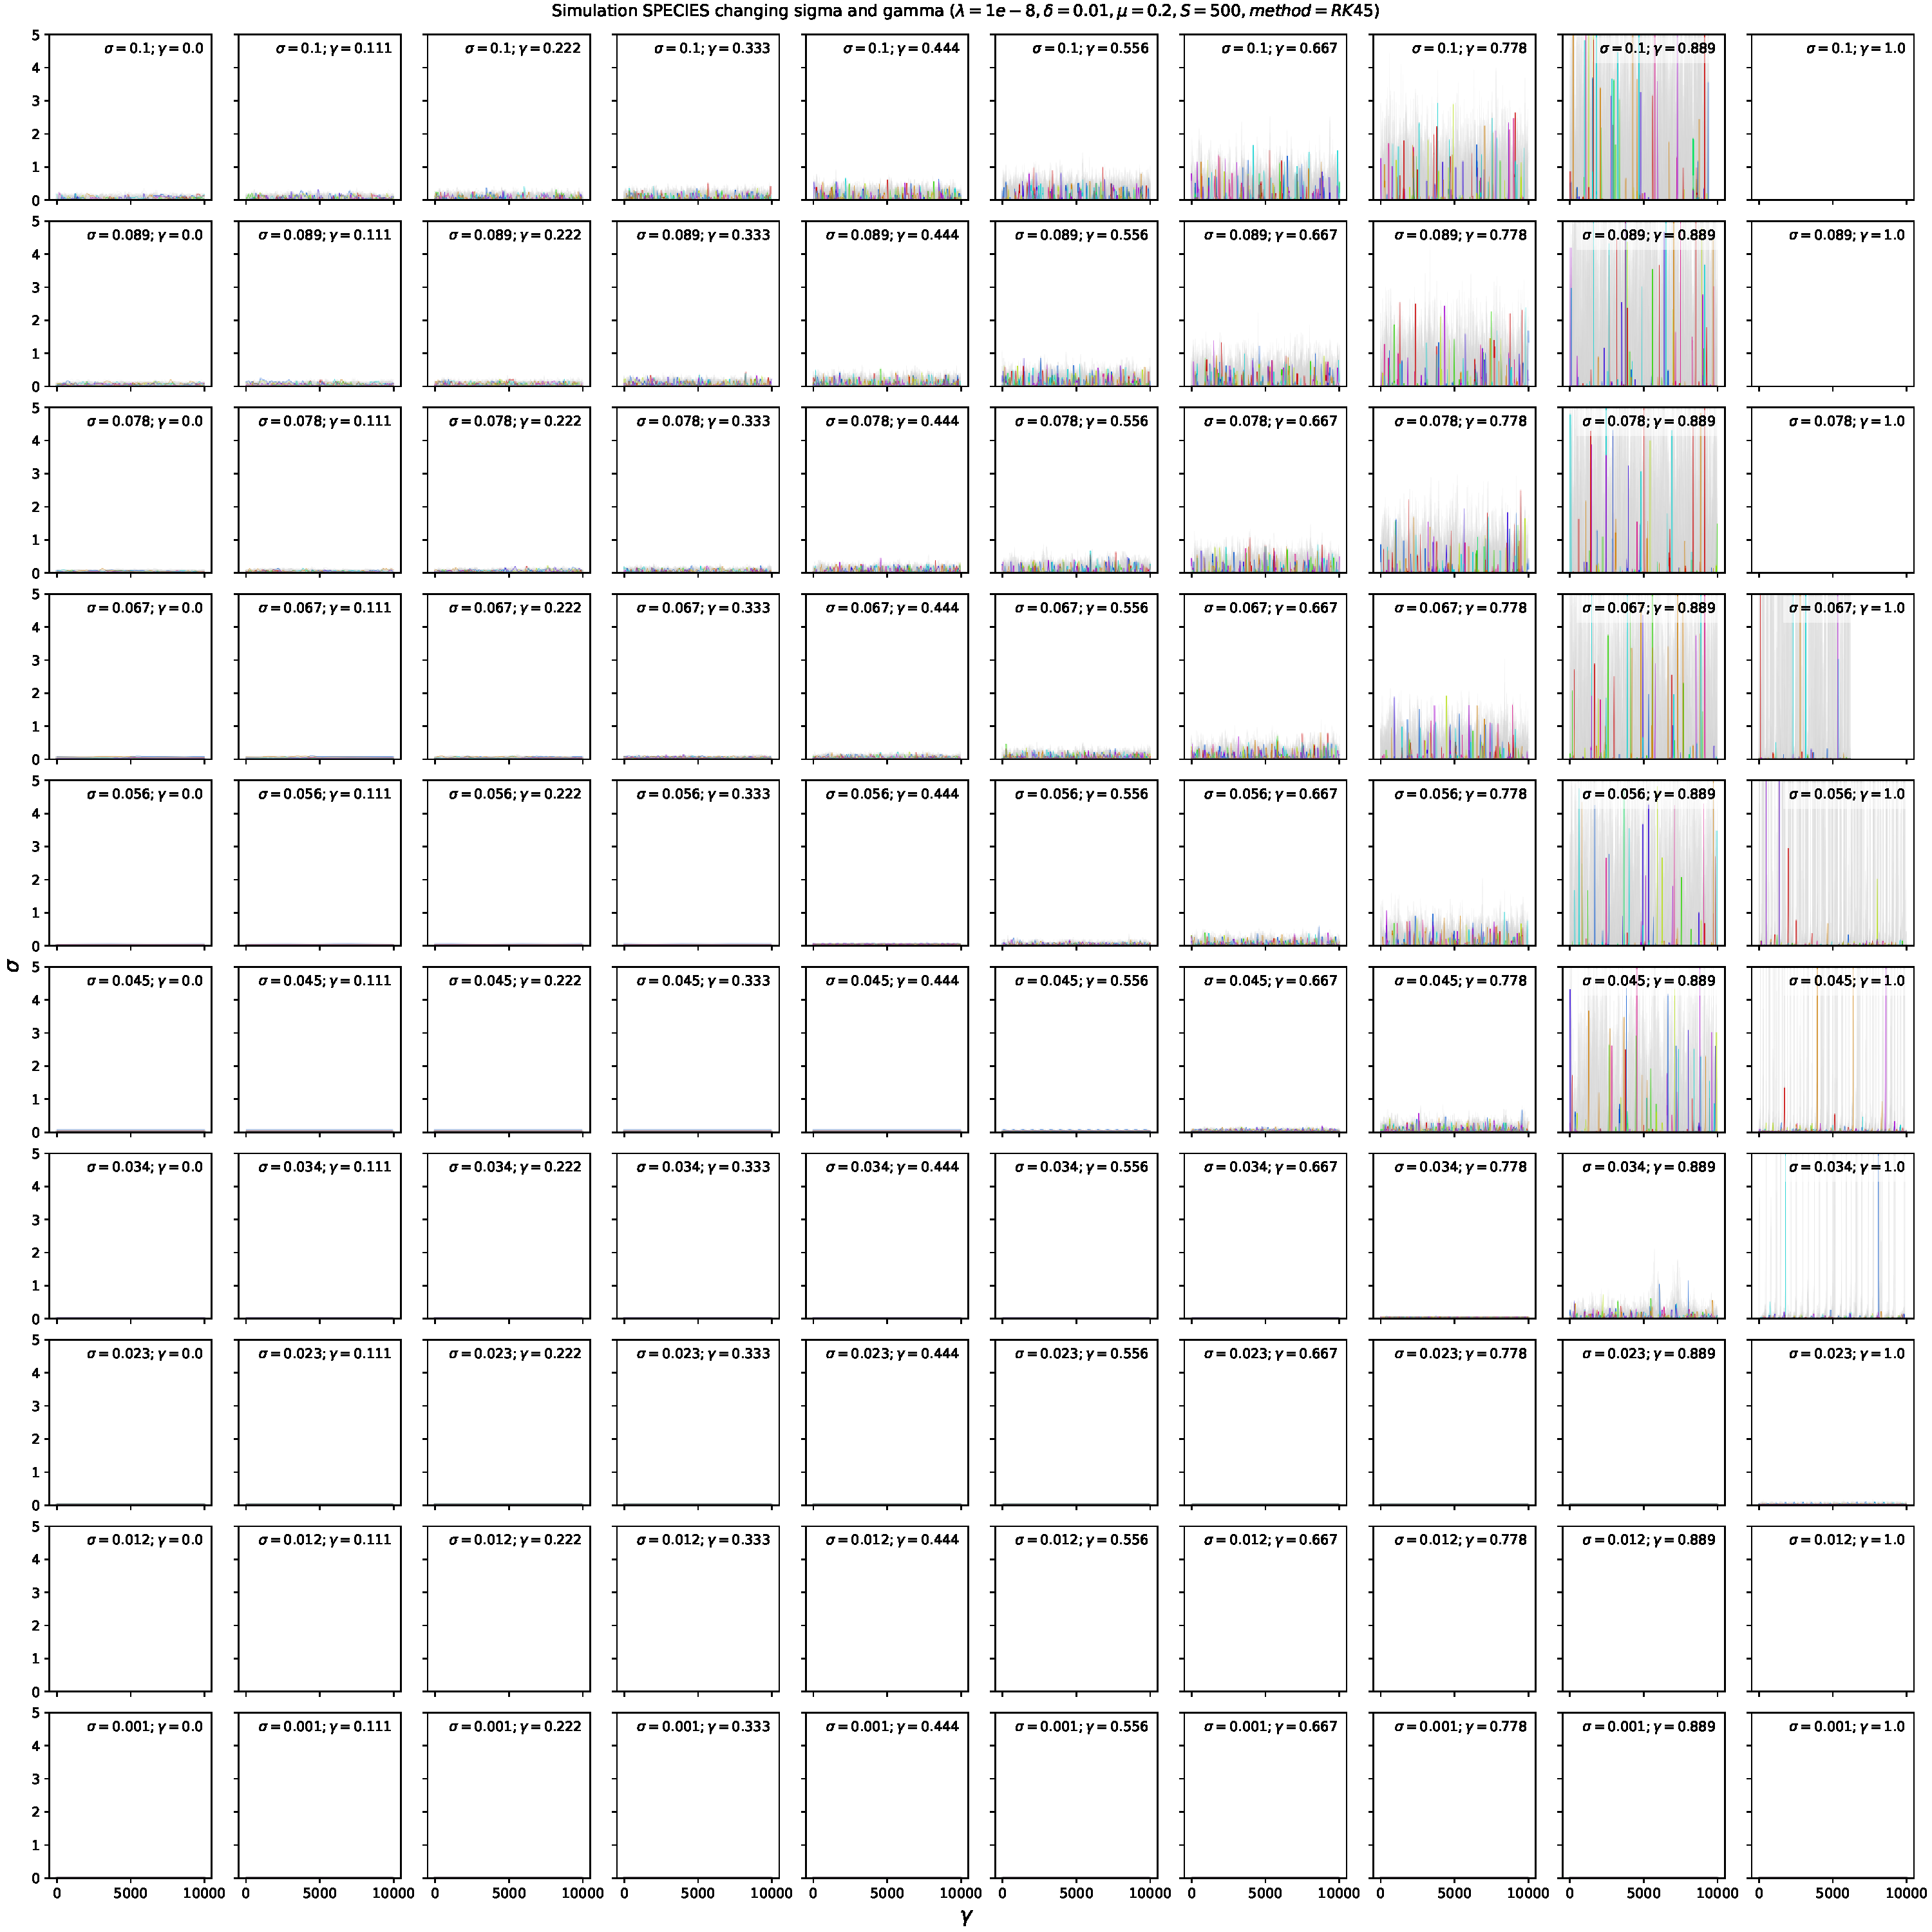
\includegraphics[width=\linewidth]{SigmaGamma/10SpeciesLinear.pdf}
    \caption{Species dynamics in linear scale $\sigma$ and $\gamma$.}
\end{figure}

\clearpage

\begin{figure}[H]
    \centering
    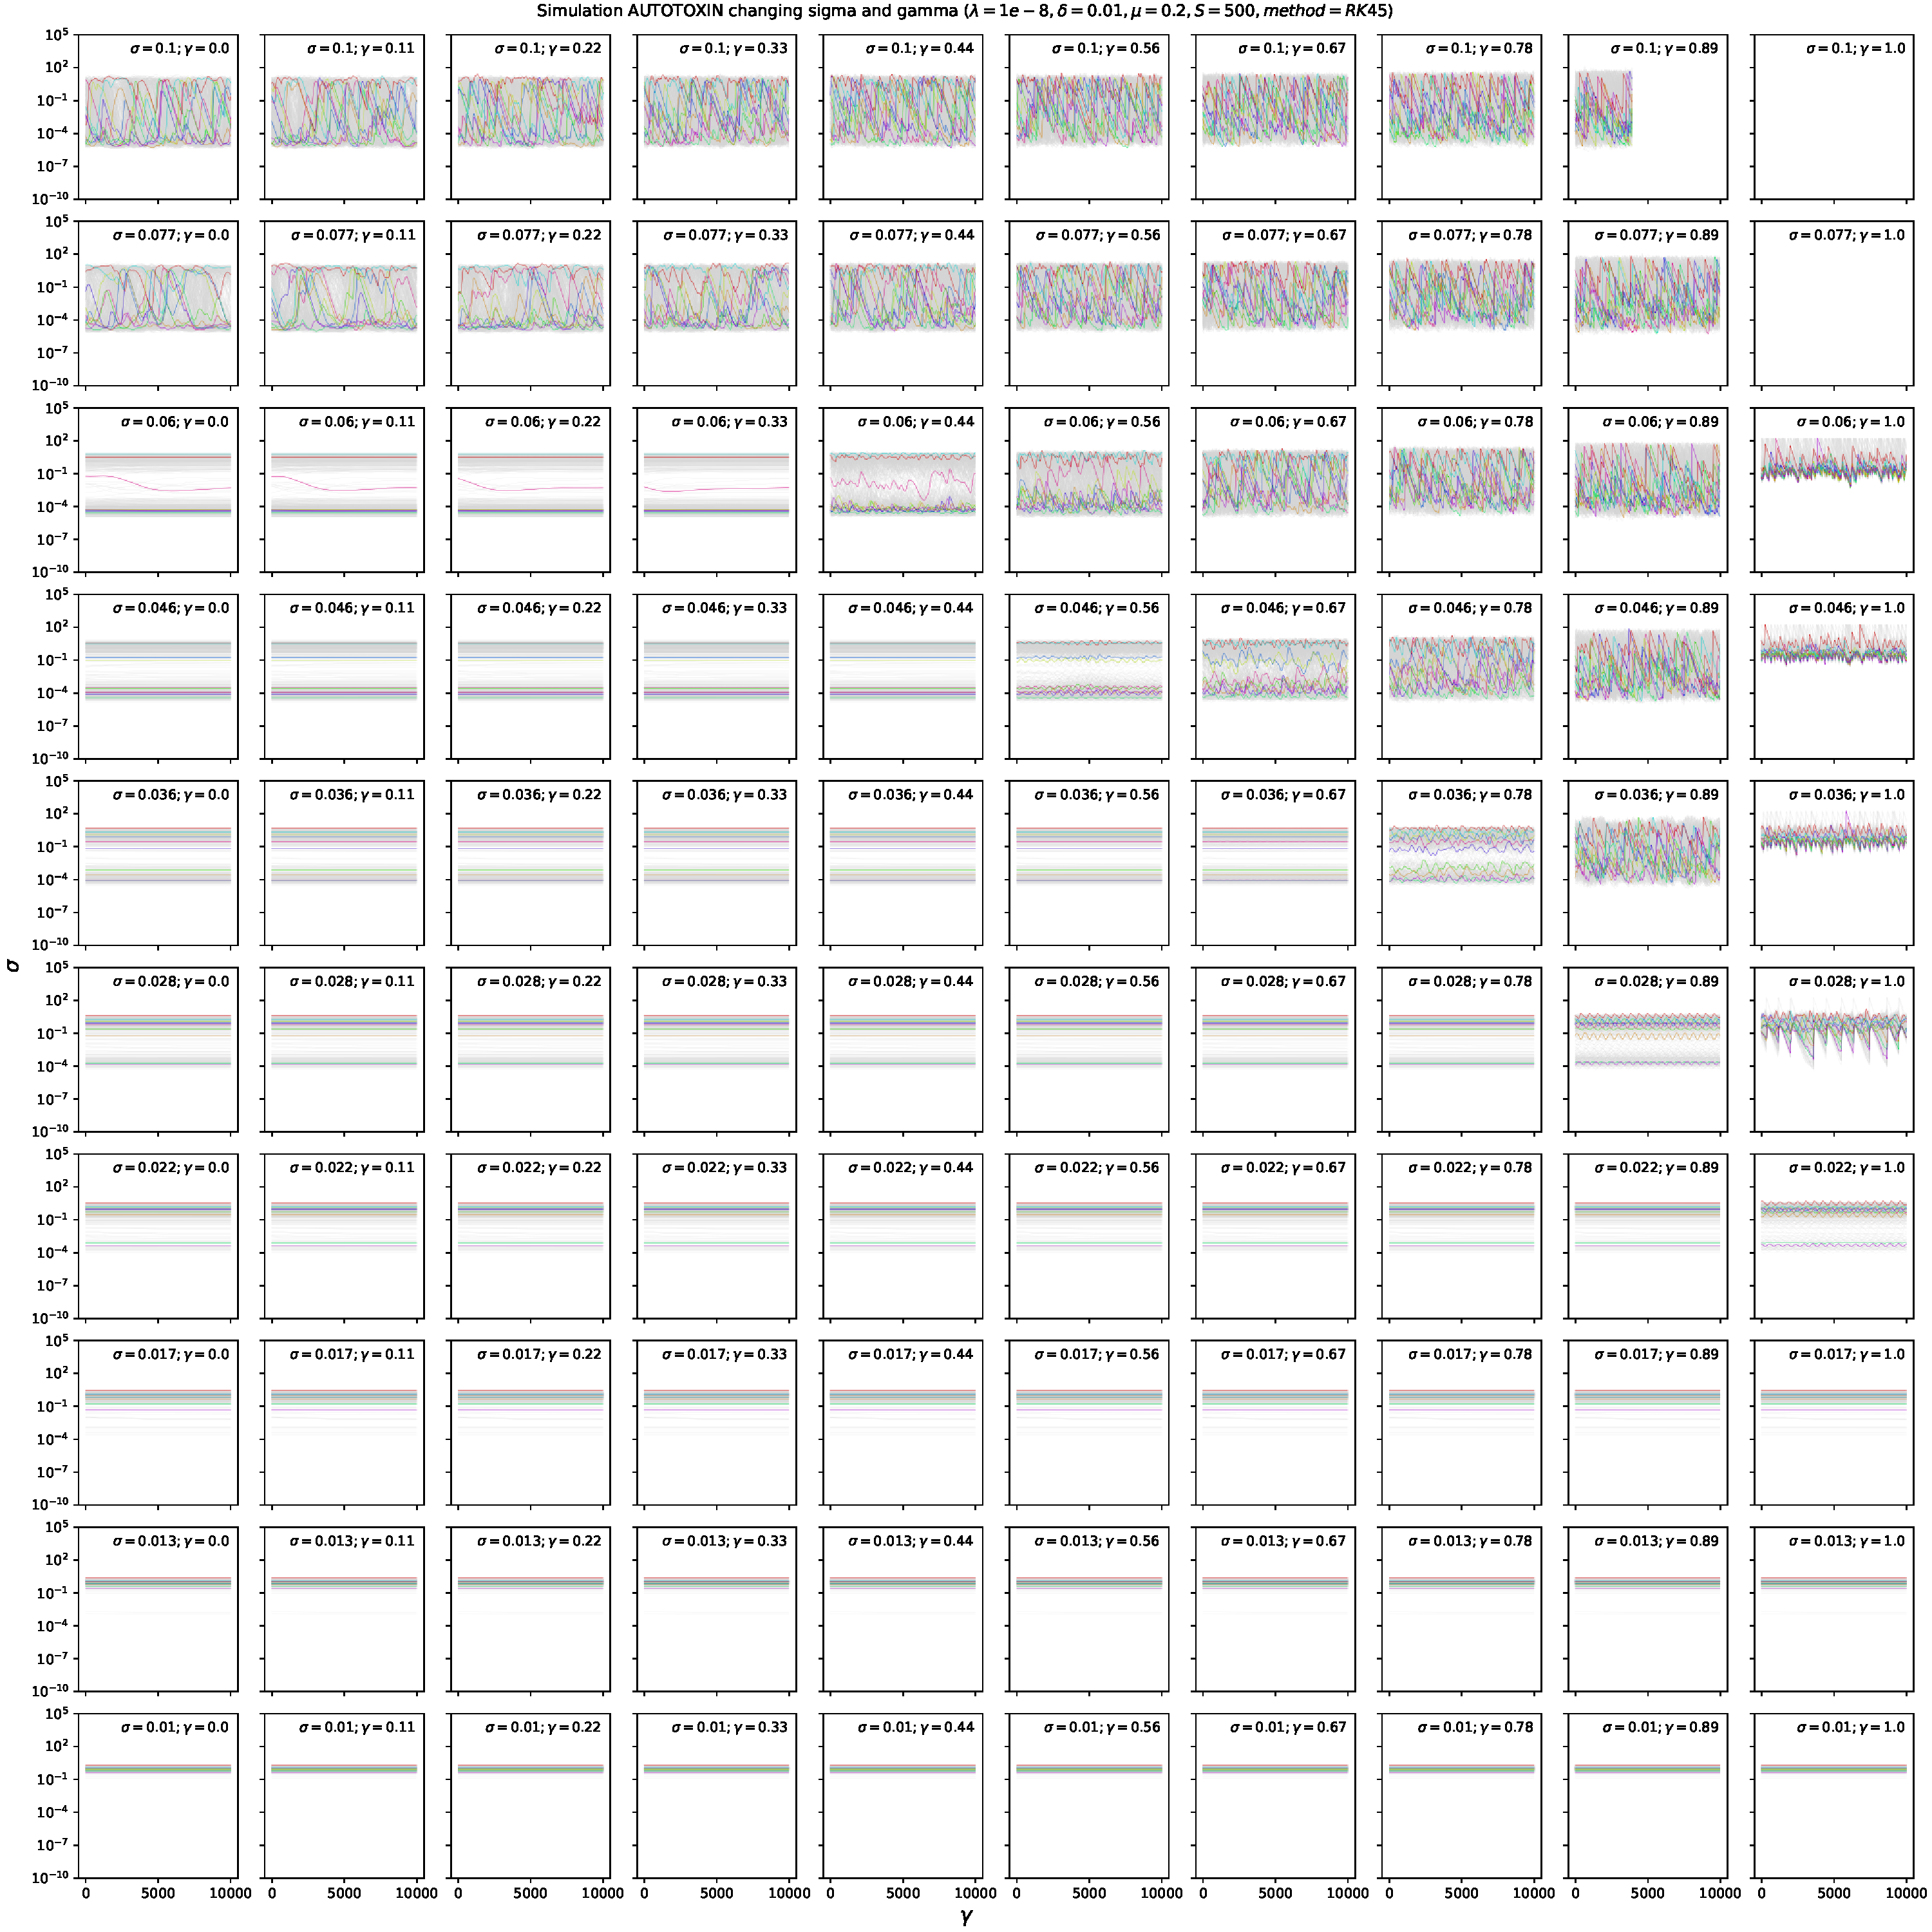
\includegraphics[width=\linewidth]{SigmaGamma/10Autotox.pdf}
    \caption{Autotoxin dynamics in logarithmic scale $\sigma$ and $\gamma$.}
\end{figure}

\clearpage

\begin{figure}[H]
    \centering
    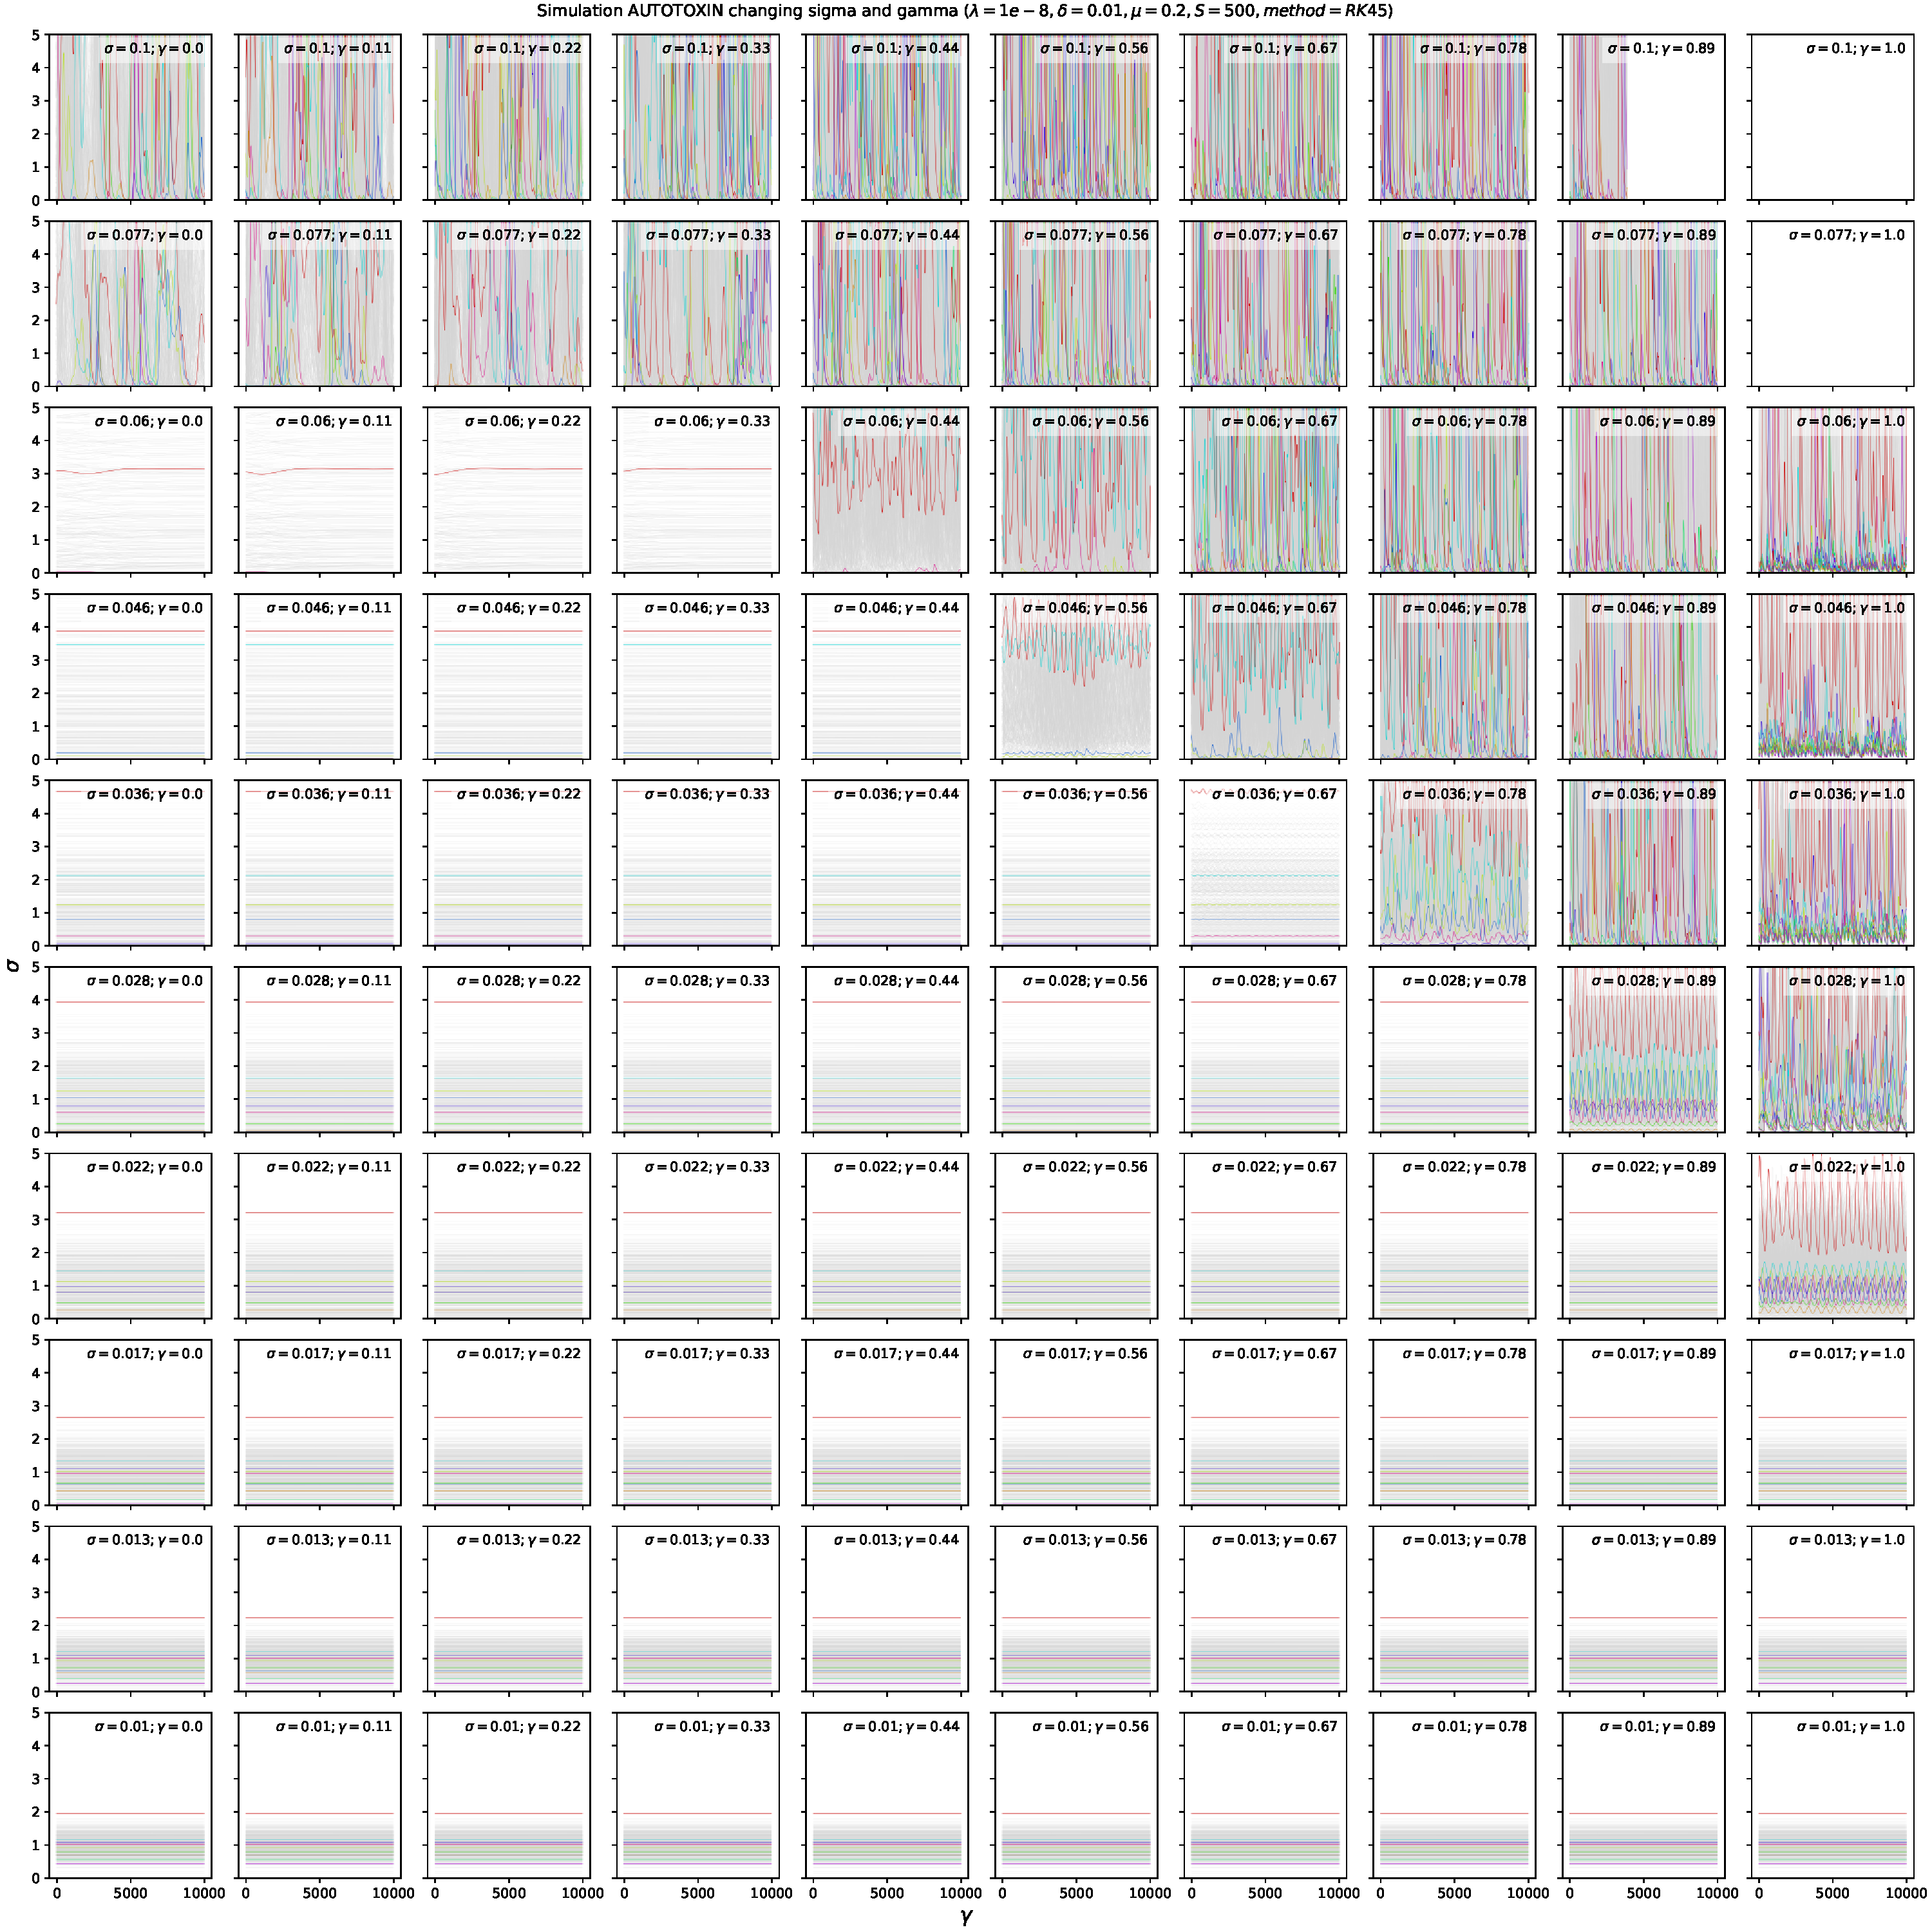
\includegraphics[width=\linewidth]{SigmaGamma/10AutotoxLinear.pdf}
    \caption{Autotoxin dynamics in linear scale $\sigma$ and $\gamma$.}
\end{figure}

\clearpage

\subsubsection{Eigen Values $\delta$–$\gamma$}

\begin{figure}[H]
    \centering
    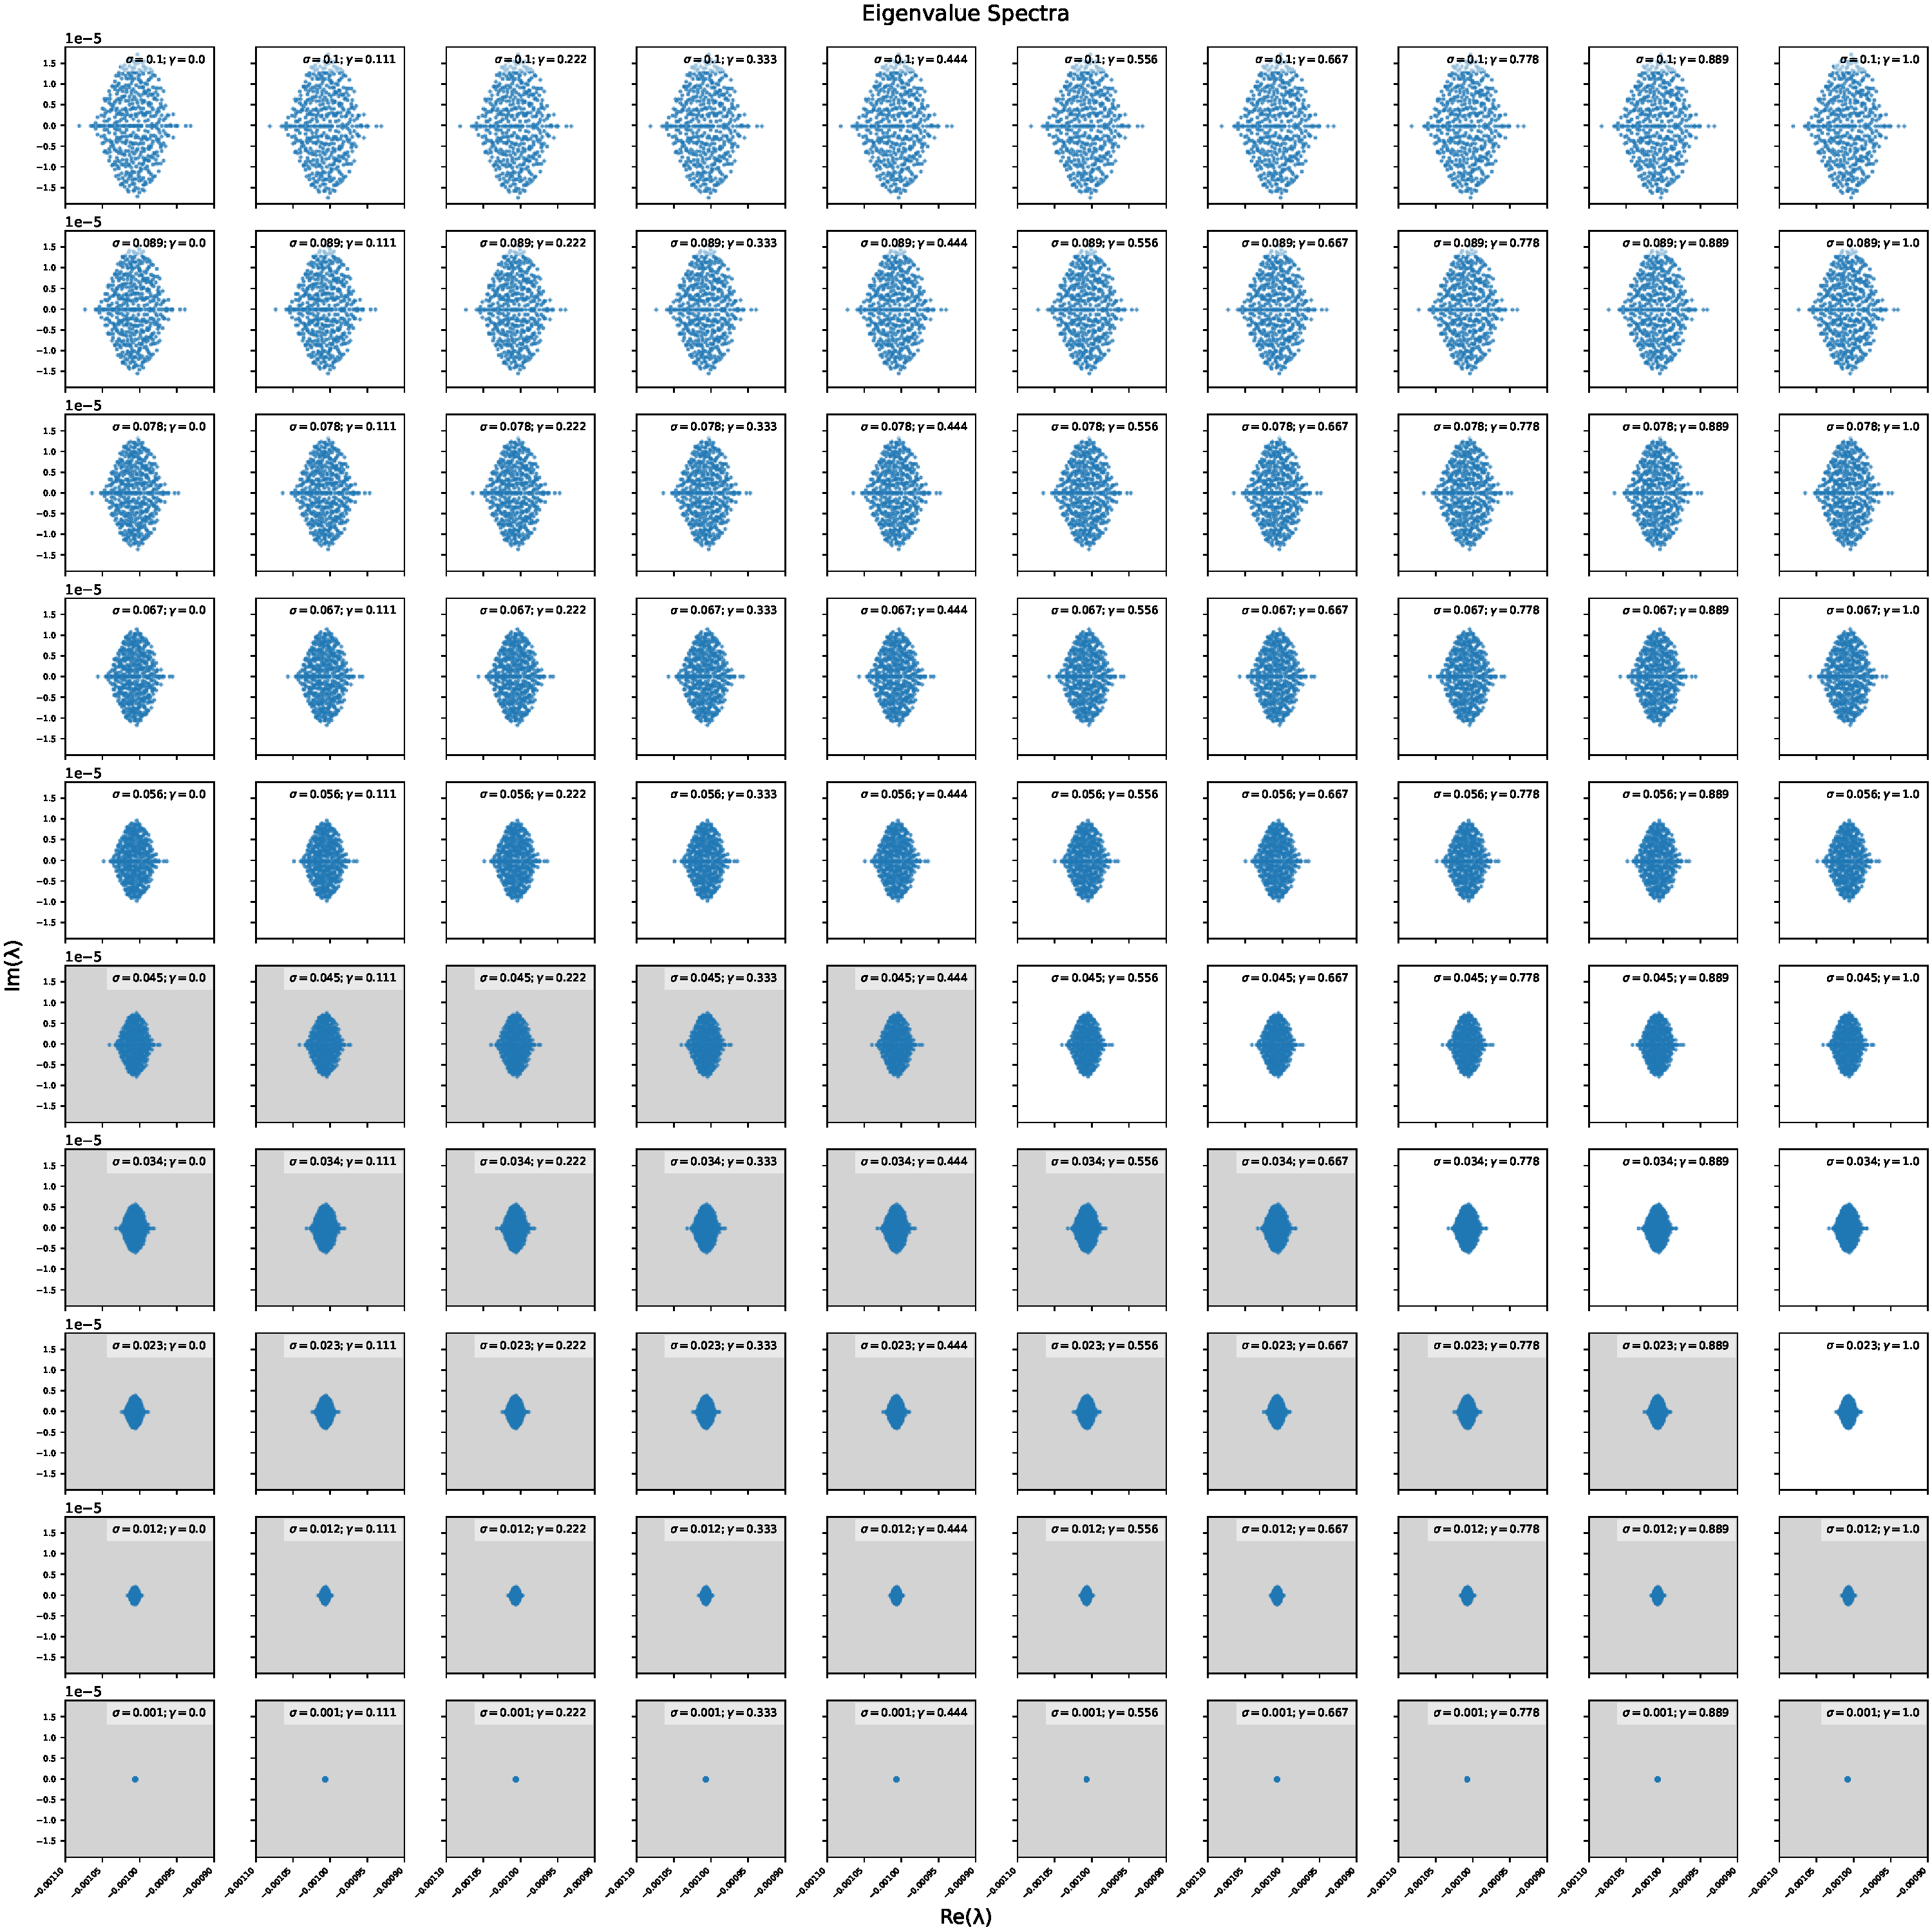
\includegraphics[width=\linewidth]{SigmaGamma/EigenvalueSpectraLog.pdf}
    \caption{Eigenvalues by changing $\sigma$ and $\gamma$.}
\end{figure}

\clearpage

\subsection{Simulations $\delta$–$\gamma$}

\[
C_{ij} \sim \mathcal{N}(0.23, 0.05), \quad 
\delta \in [0.001, 1], \quad 
\gamma \in [0, 1], \quad \lambda = 10^{-8}
\]

\begin{figure}[H]
    \centering
    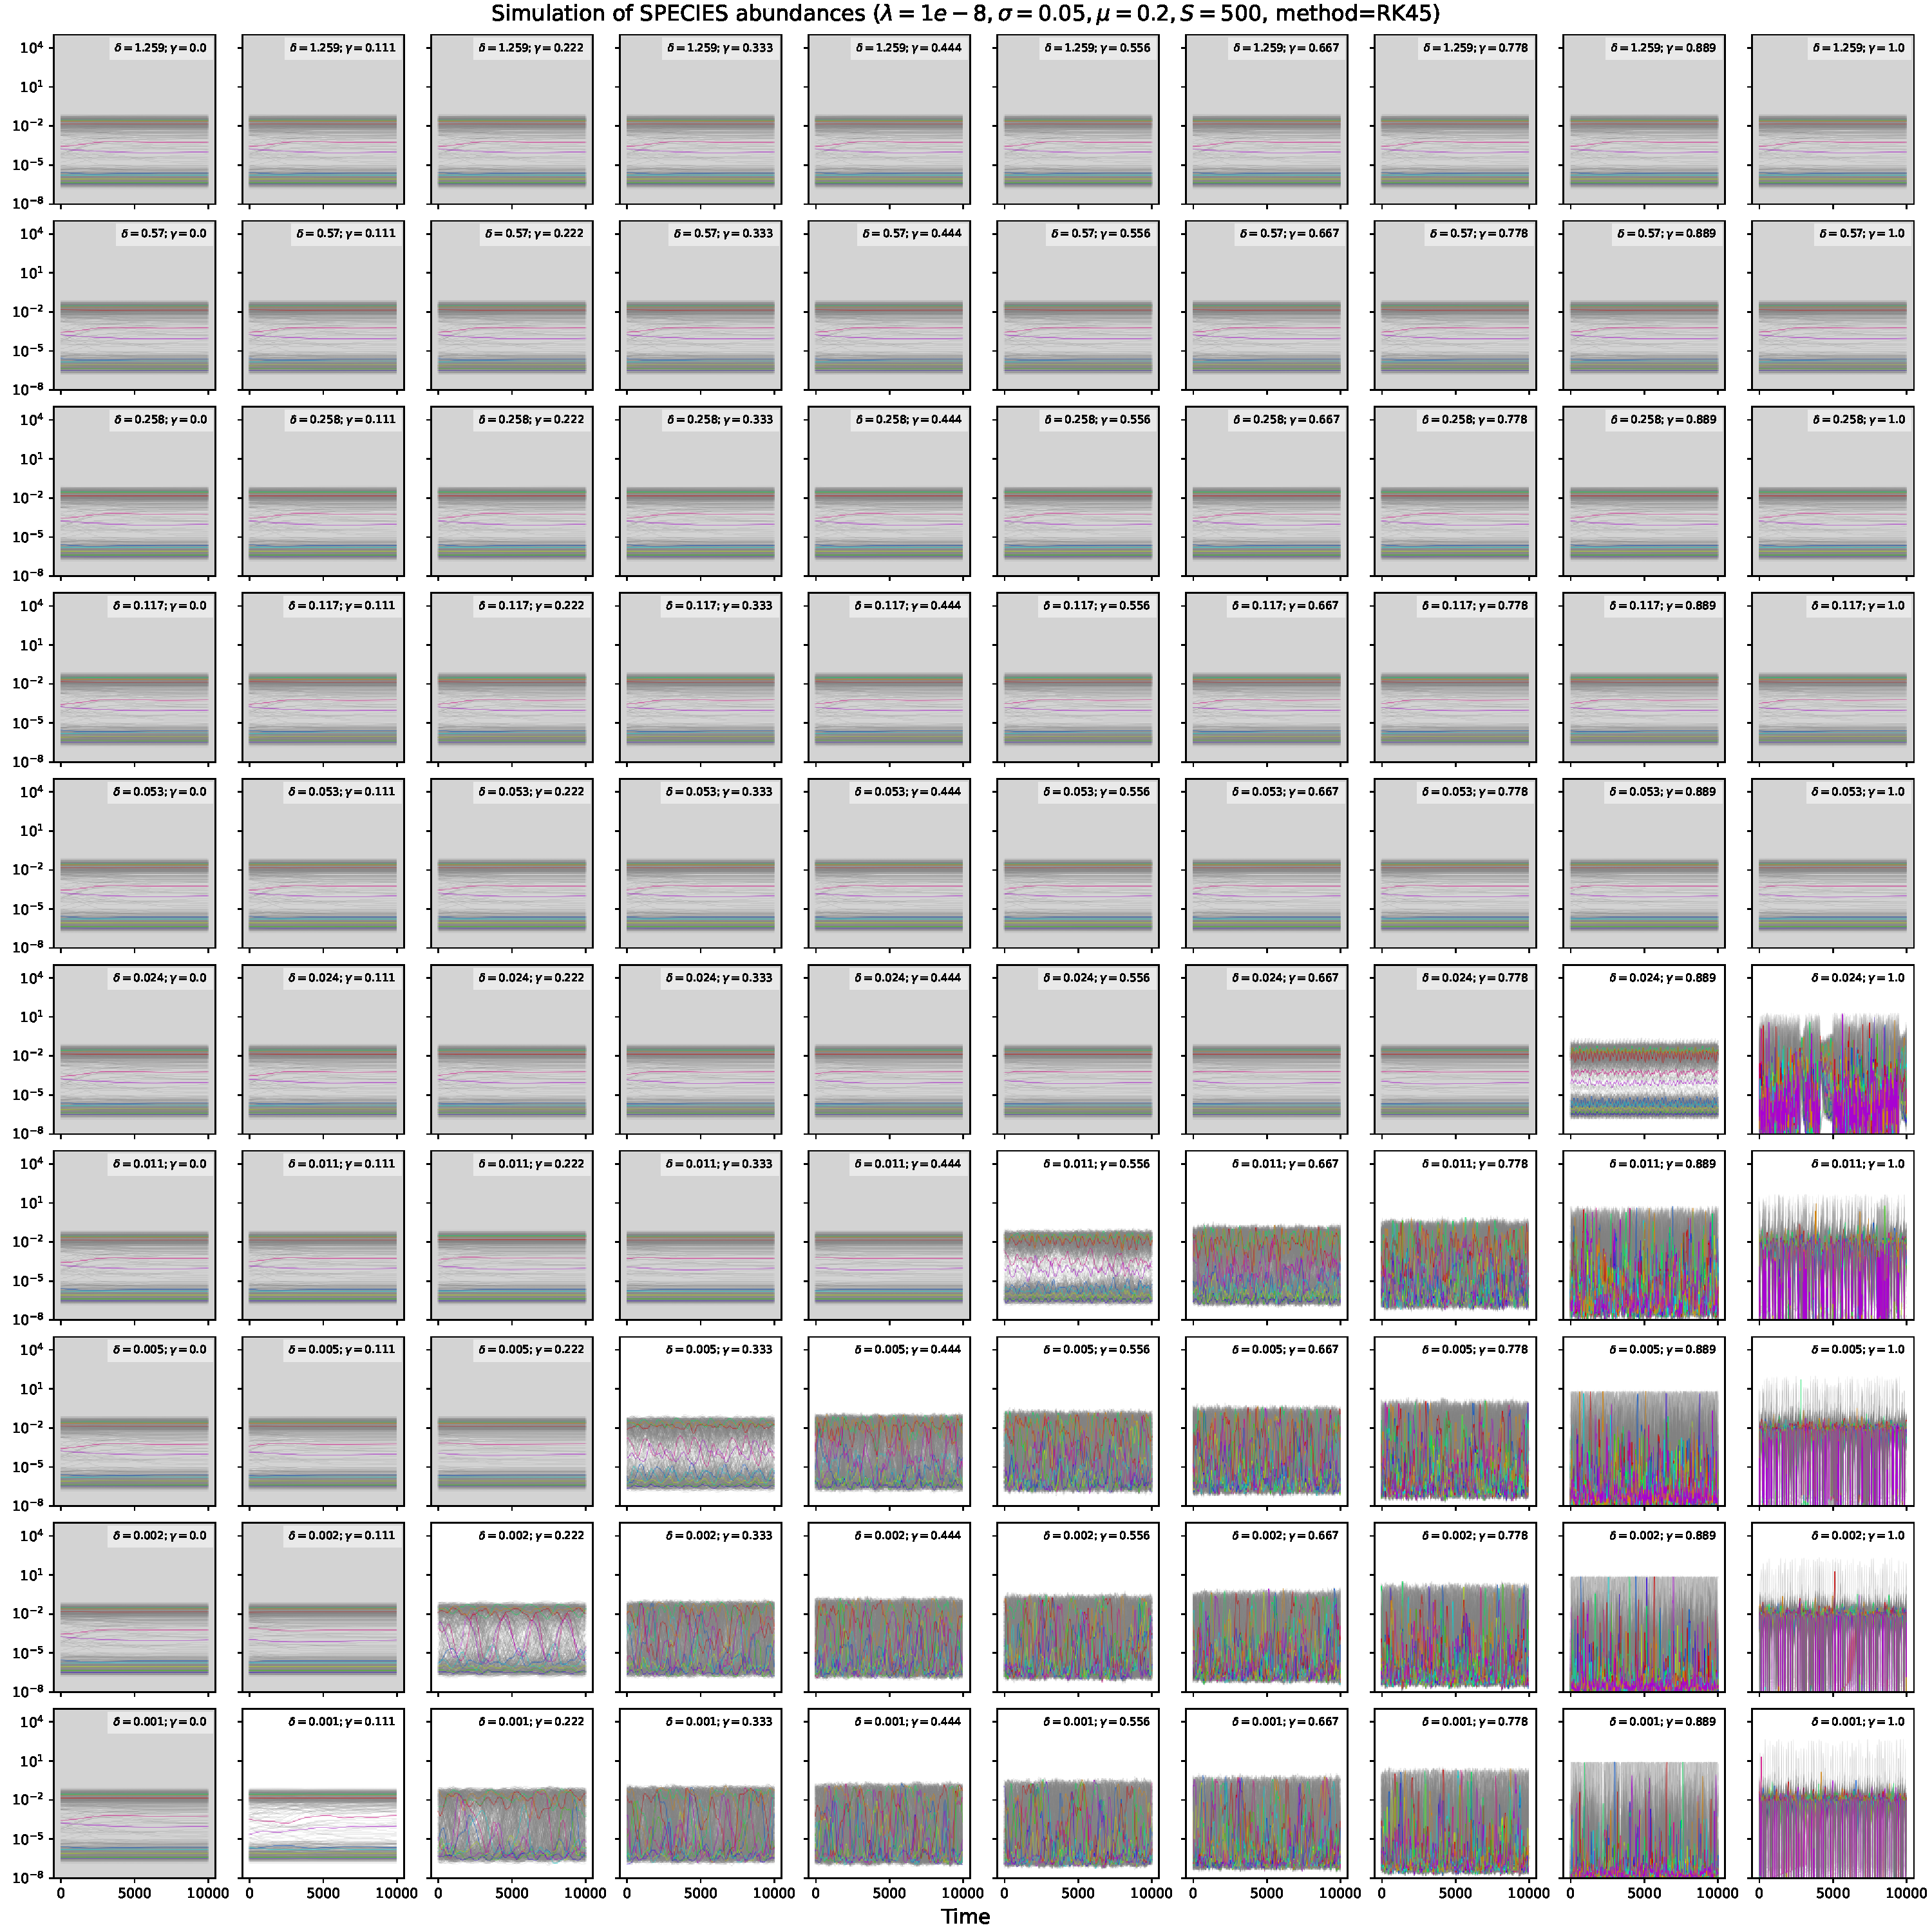
\includegraphics[width=\linewidth]{DeltaGamma/10Species.pdf}
    \caption{Species dynamics in logarithmic scale changing $\delta$ and $\gamma$.}
\end{figure}

\clearpage

\begin{figure}[H]
    \centering
    \includegraphics[width=\linewidth]{DeltaGamma/10SpeciesFPLinear.pdf}
    \caption{Species dynamics in linear scale changing $\delta$ and $\gamma$.}
\end{figure}

\clearpage

\begin{figure}[H]
    \centering
    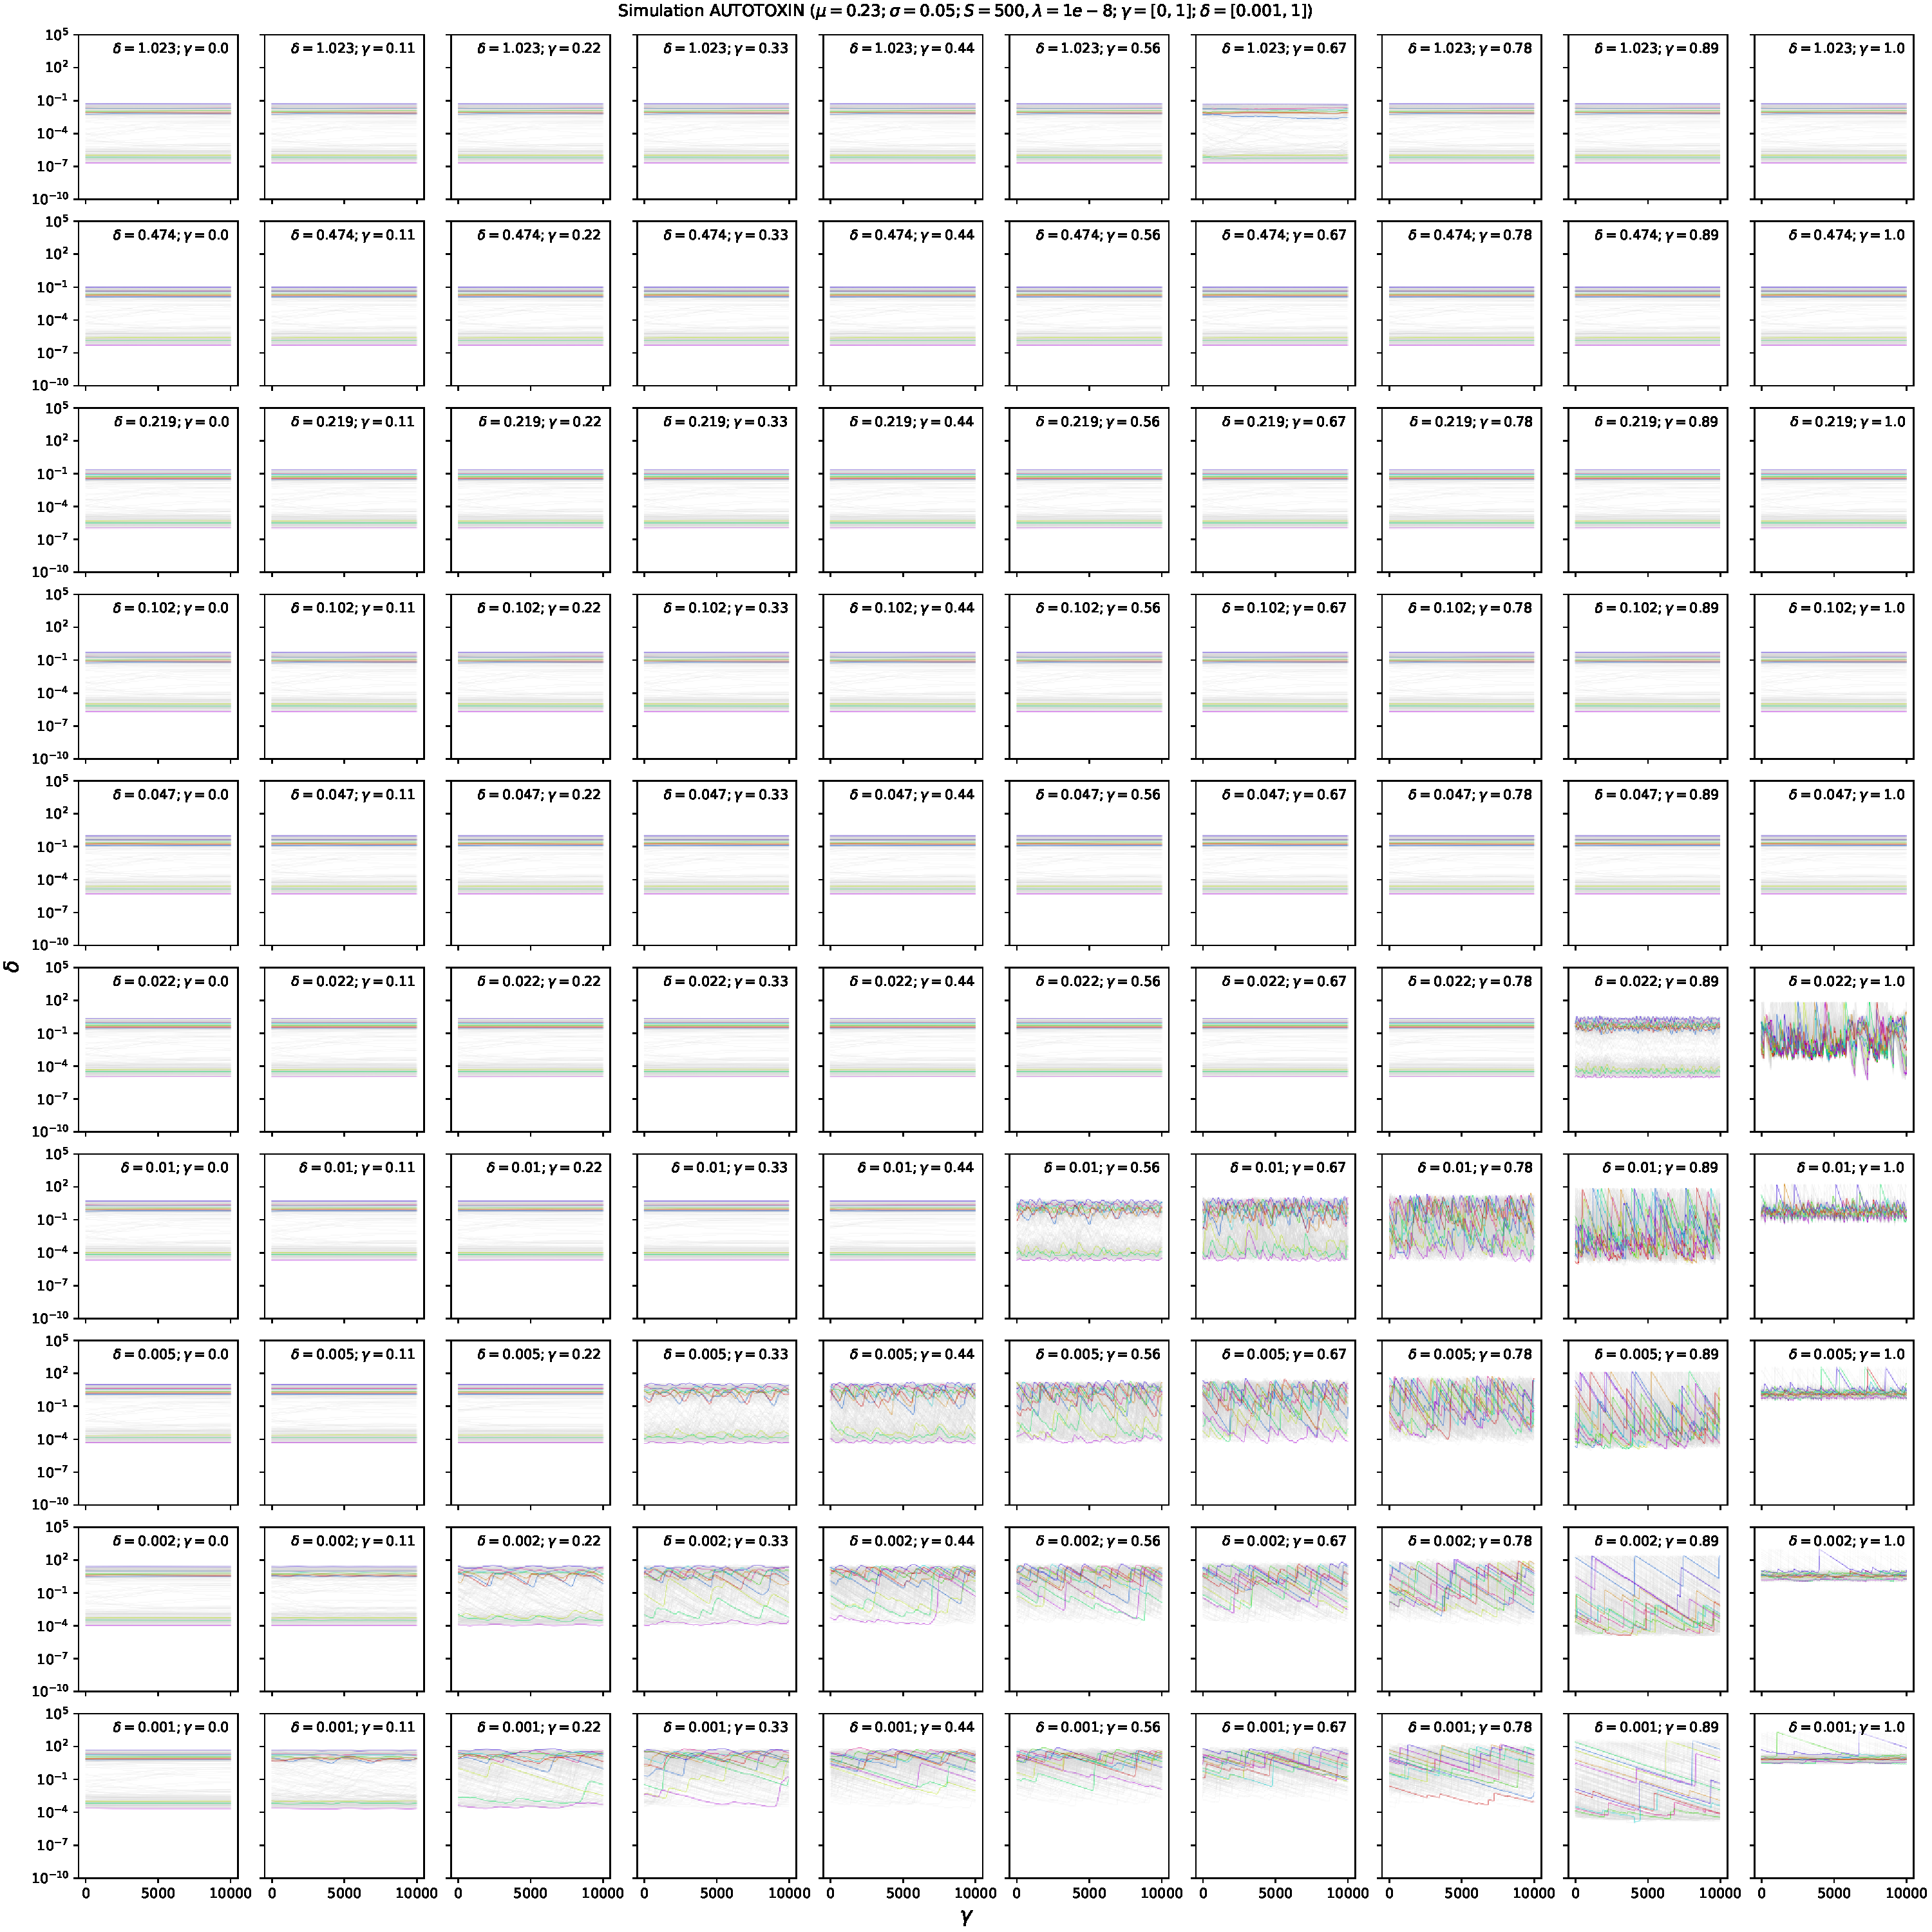
\includegraphics[width=\linewidth]{DeltaGamma/10autotoxFP.pdf}
    \caption{Autotoxin dynamics in logarithmic scale changing $\delta$ and $\gamma$.}
\end{figure}

\clearpage

\begin{figure}[H]
    \centering
    \includegraphics[width=\linewidth]{DeltaGamma/10AutotoxFPLinear.pdf}
    \caption{Autotoxin dynamics in linear scale changing $\delta$ and $\gamma$.}
\end{figure}

\clearpage

\begin{figure}[H]
    \centering
    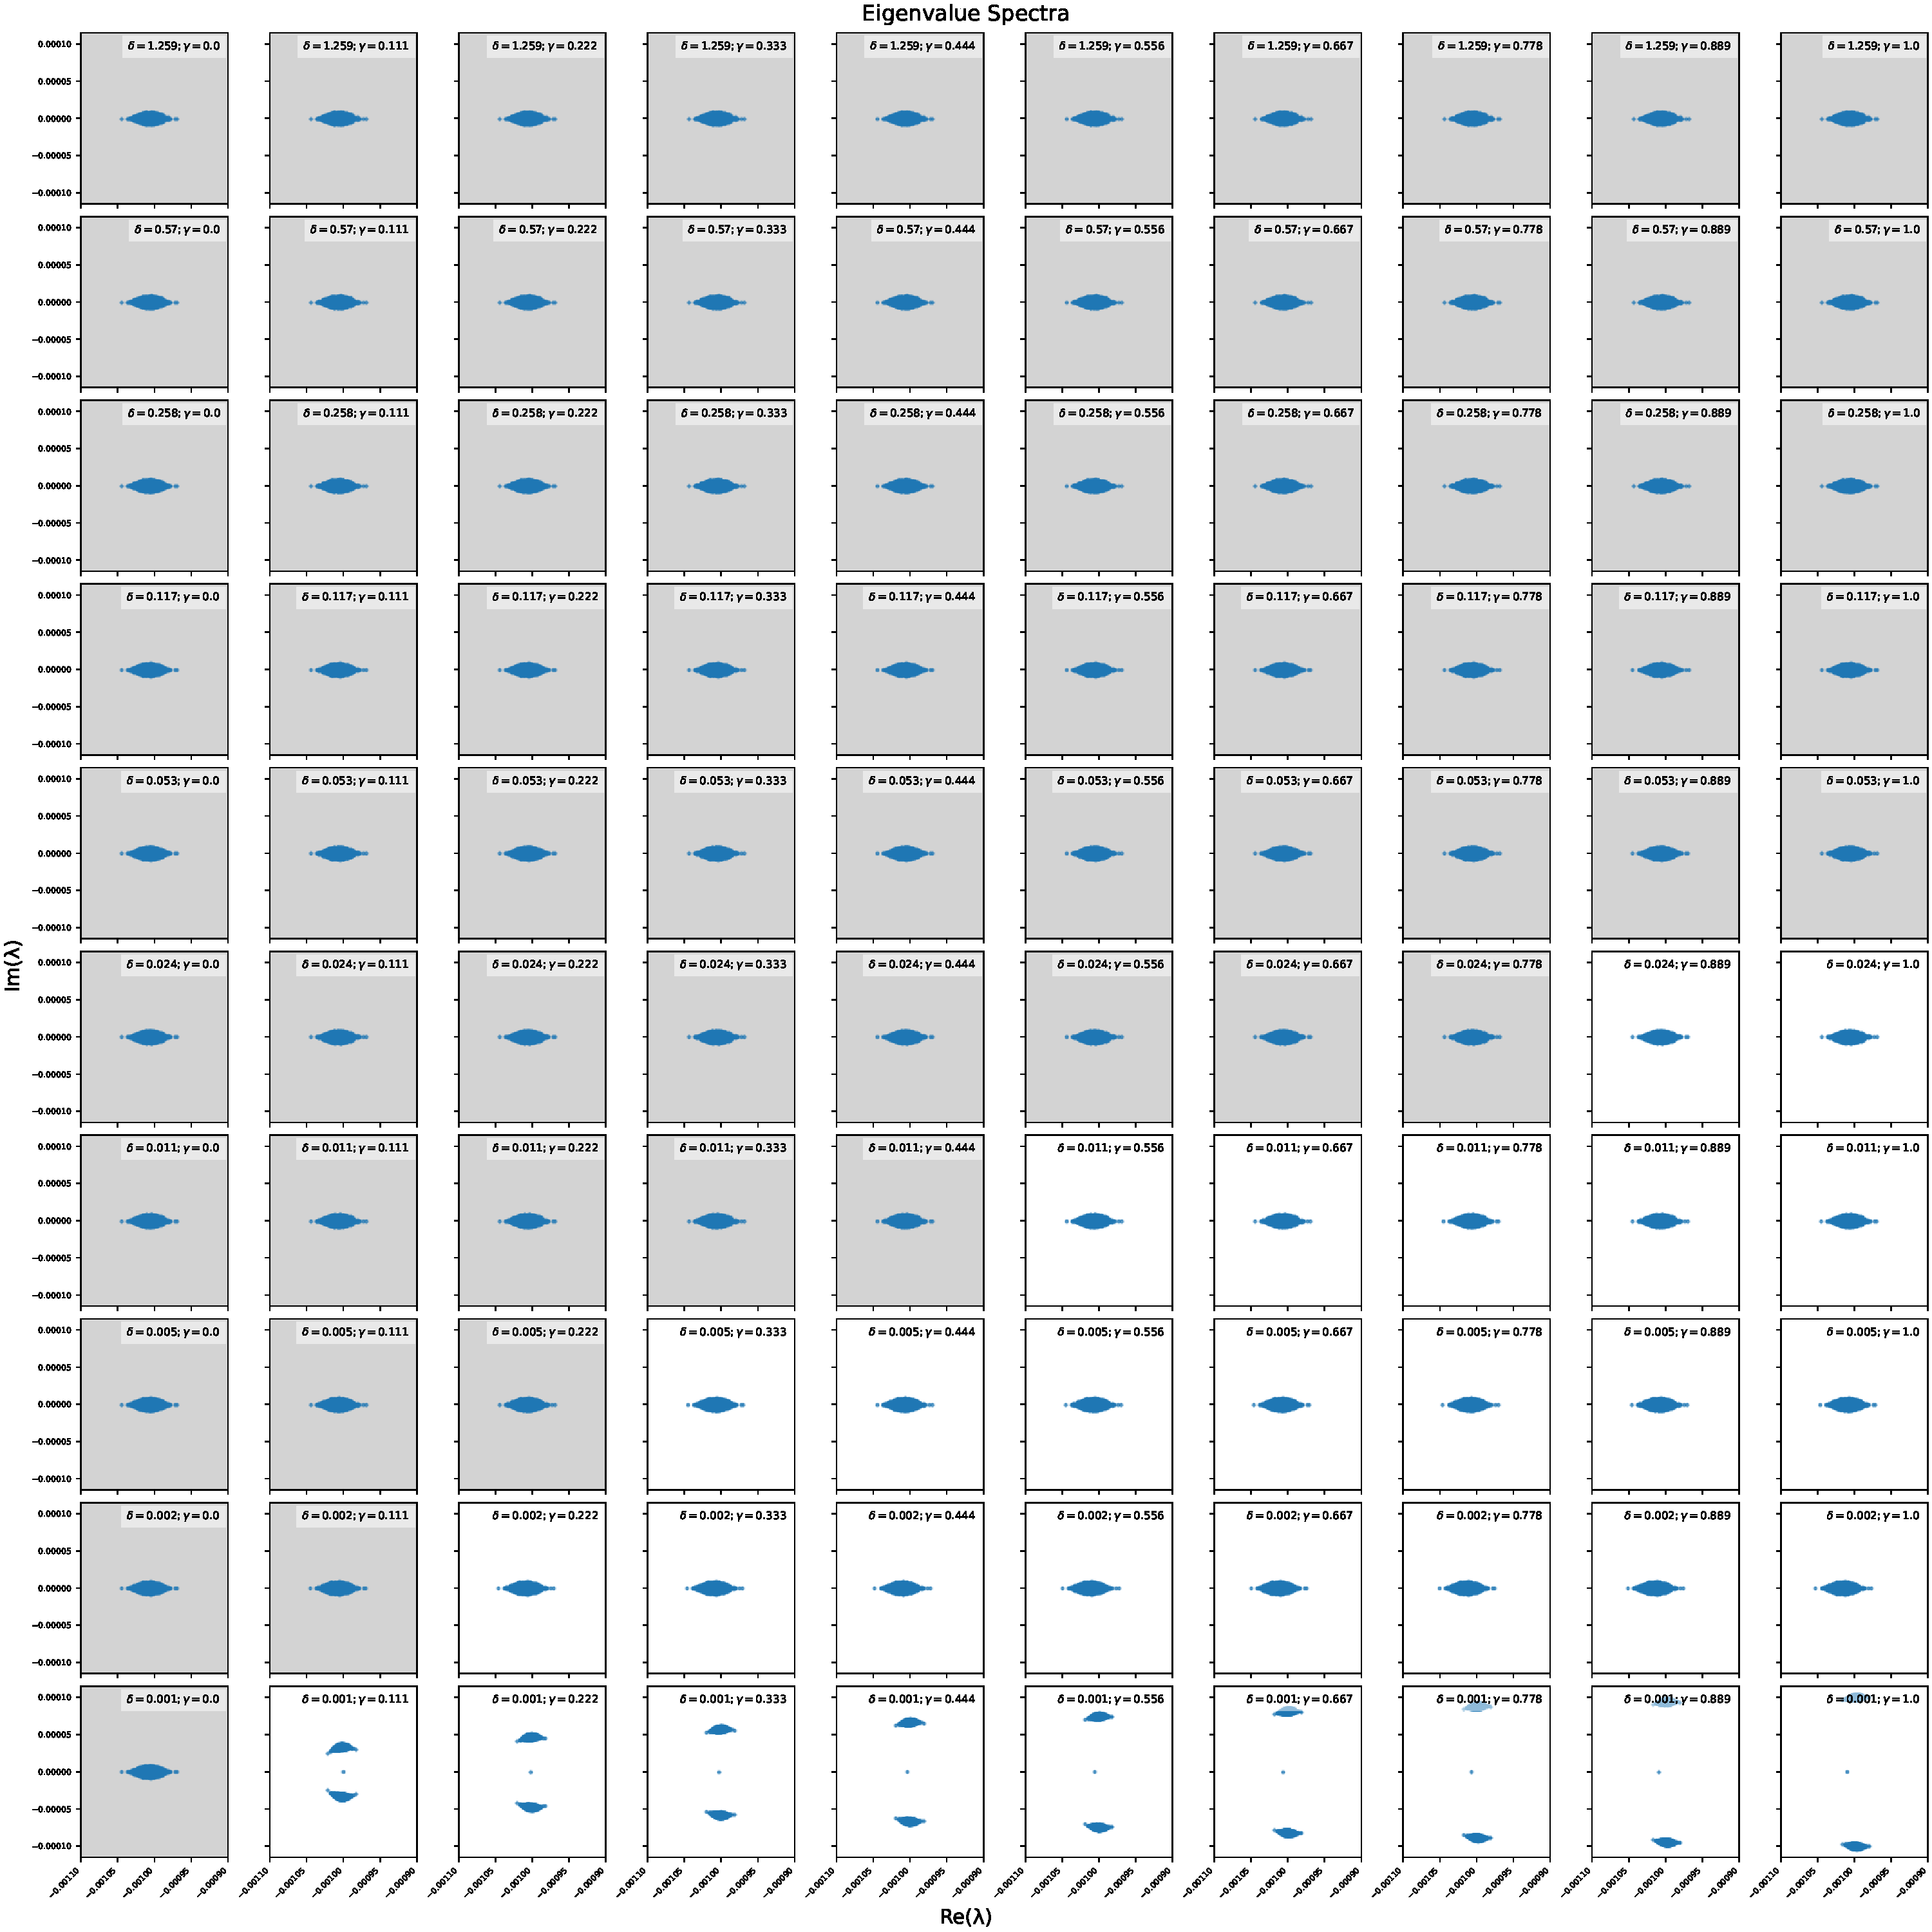
\includegraphics[width=\linewidth]{DeltaGamma/EigenvalueSpectraLog.pdf}
    \caption{Eigenvalues by changing $\delta$ and $\gamma$.}
\end{figure}

\clearpage


\subsection{Bifurcation Analysis}

\subsubsection{Varying $\gamma$ from 0 to 0.89}

\begin{figure}[H]
    \centering
    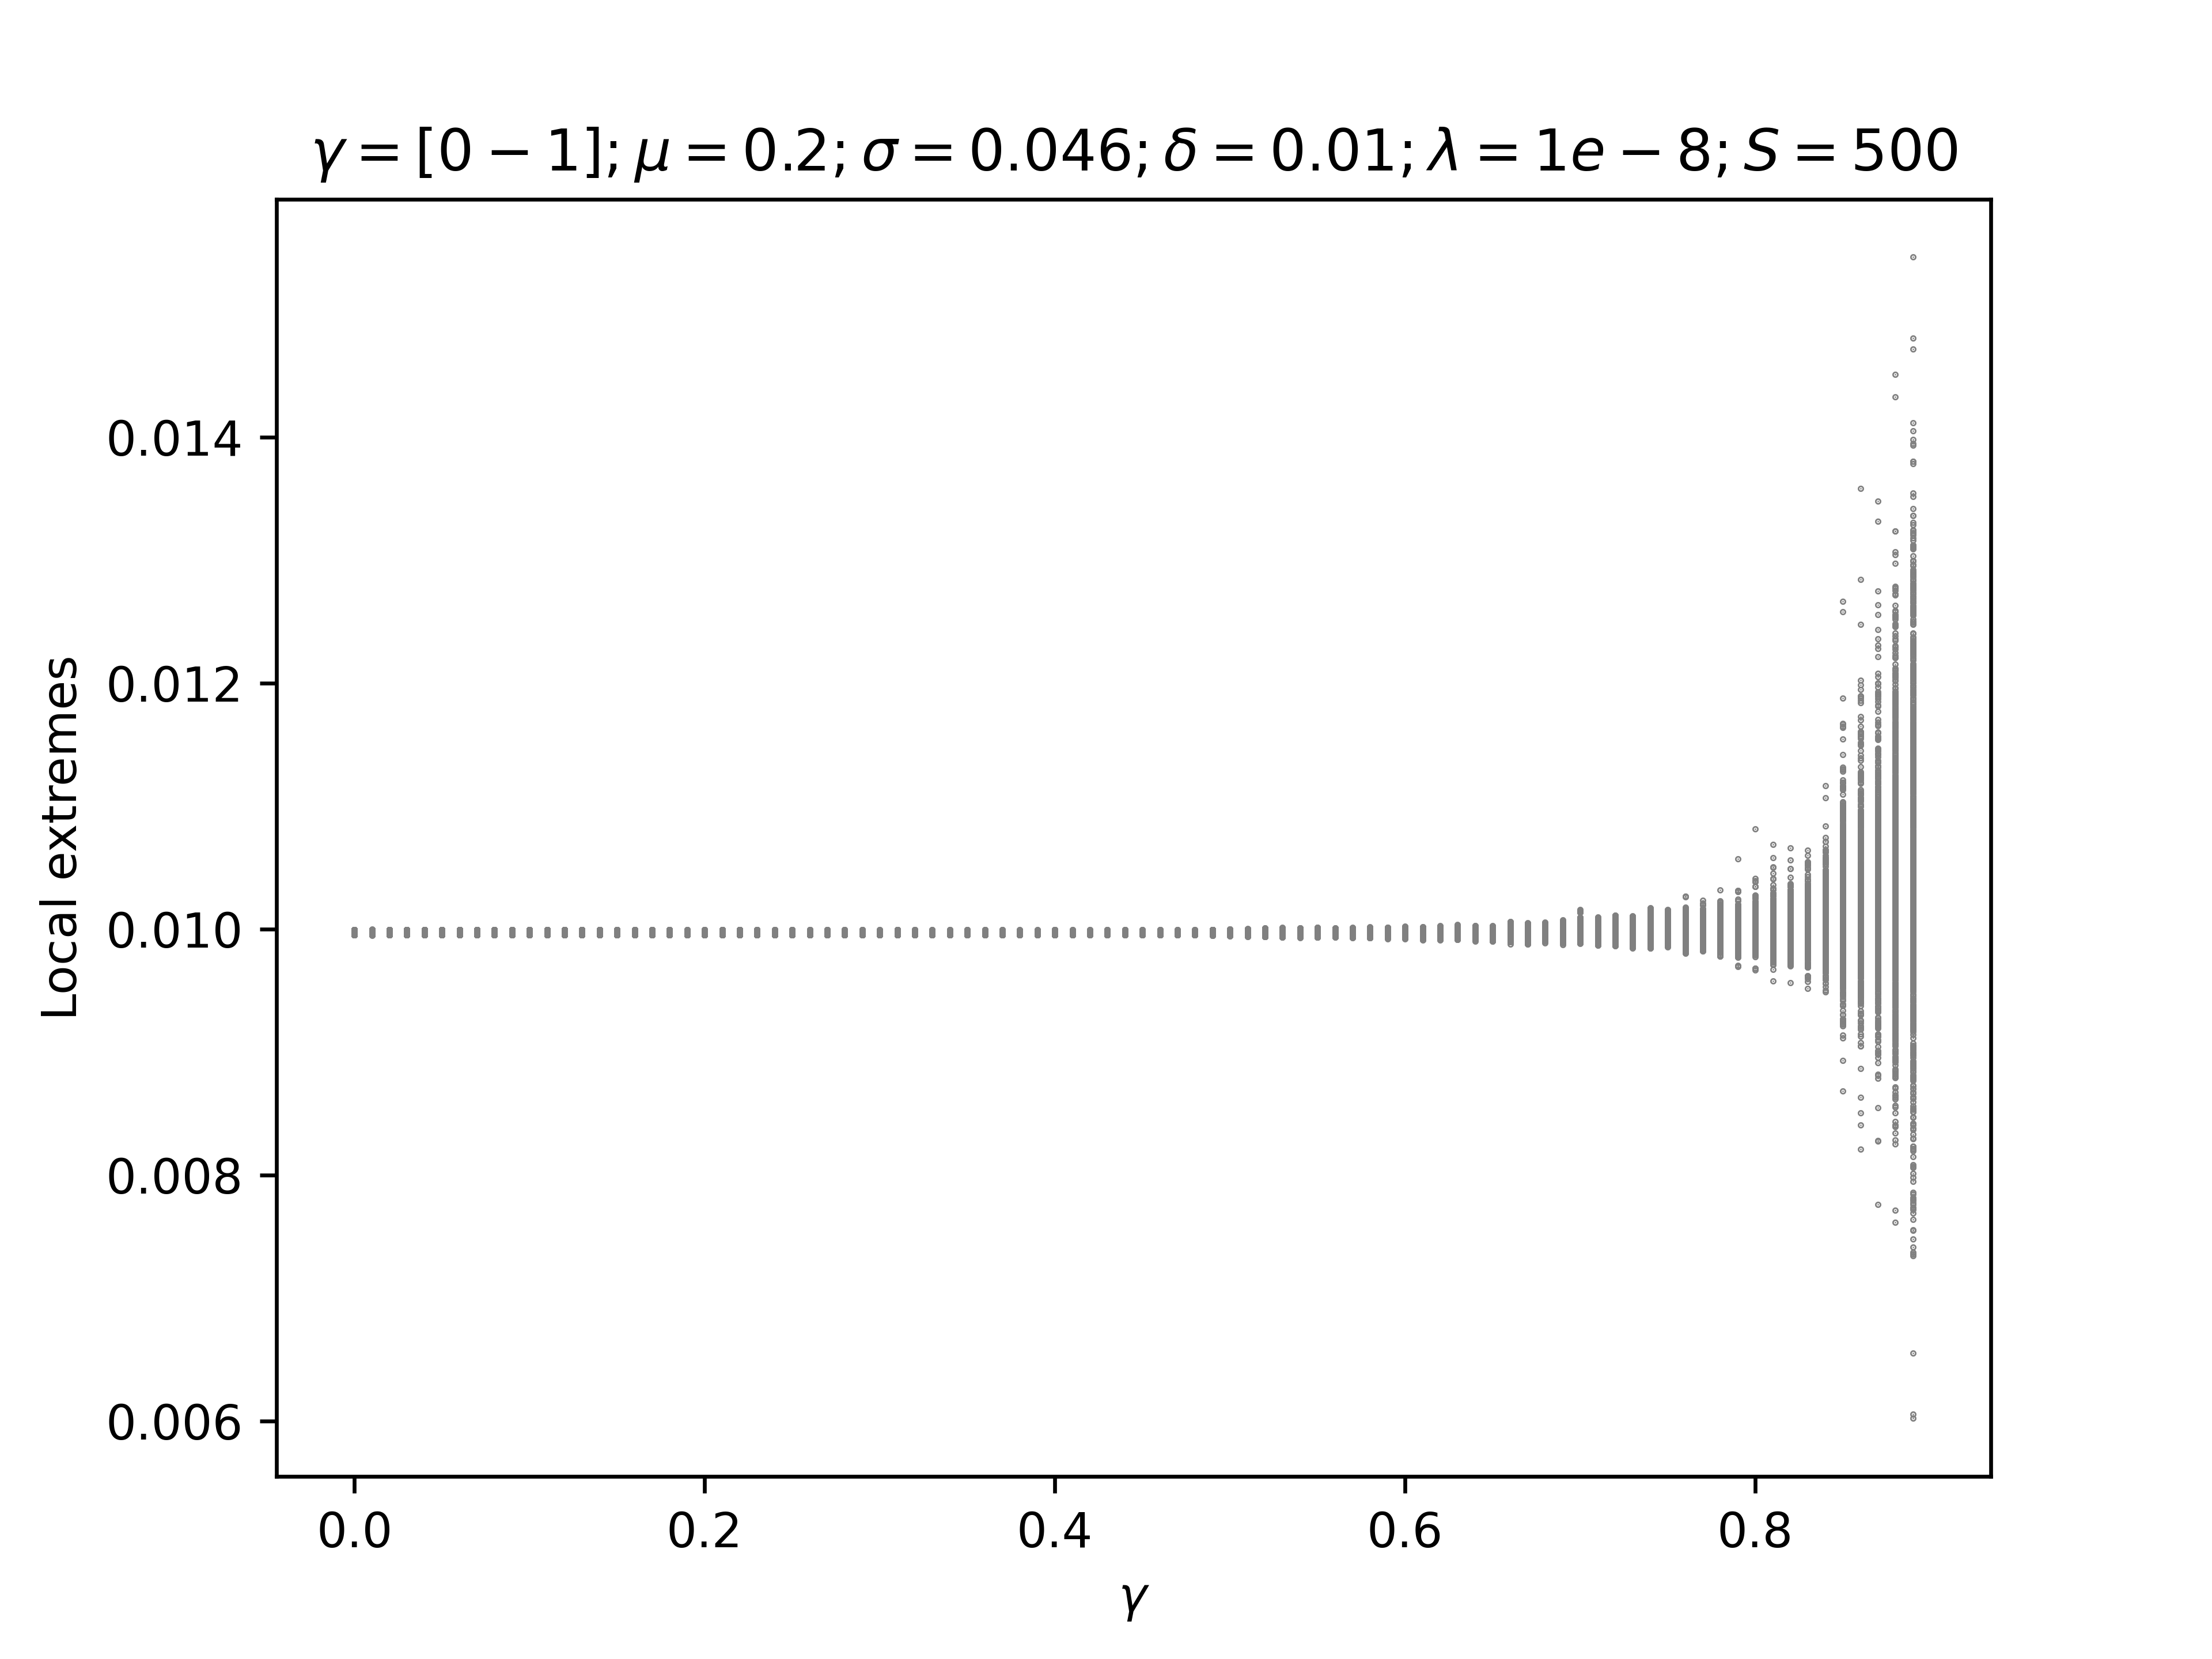
\includegraphics[width=\linewidth]{Bifurcation/BifurcationMeanGamma.png}
    \caption{Mean abundance of all species as a function of $\gamma$.}
\end{figure}

\begin{figure}[H]
    \centering
    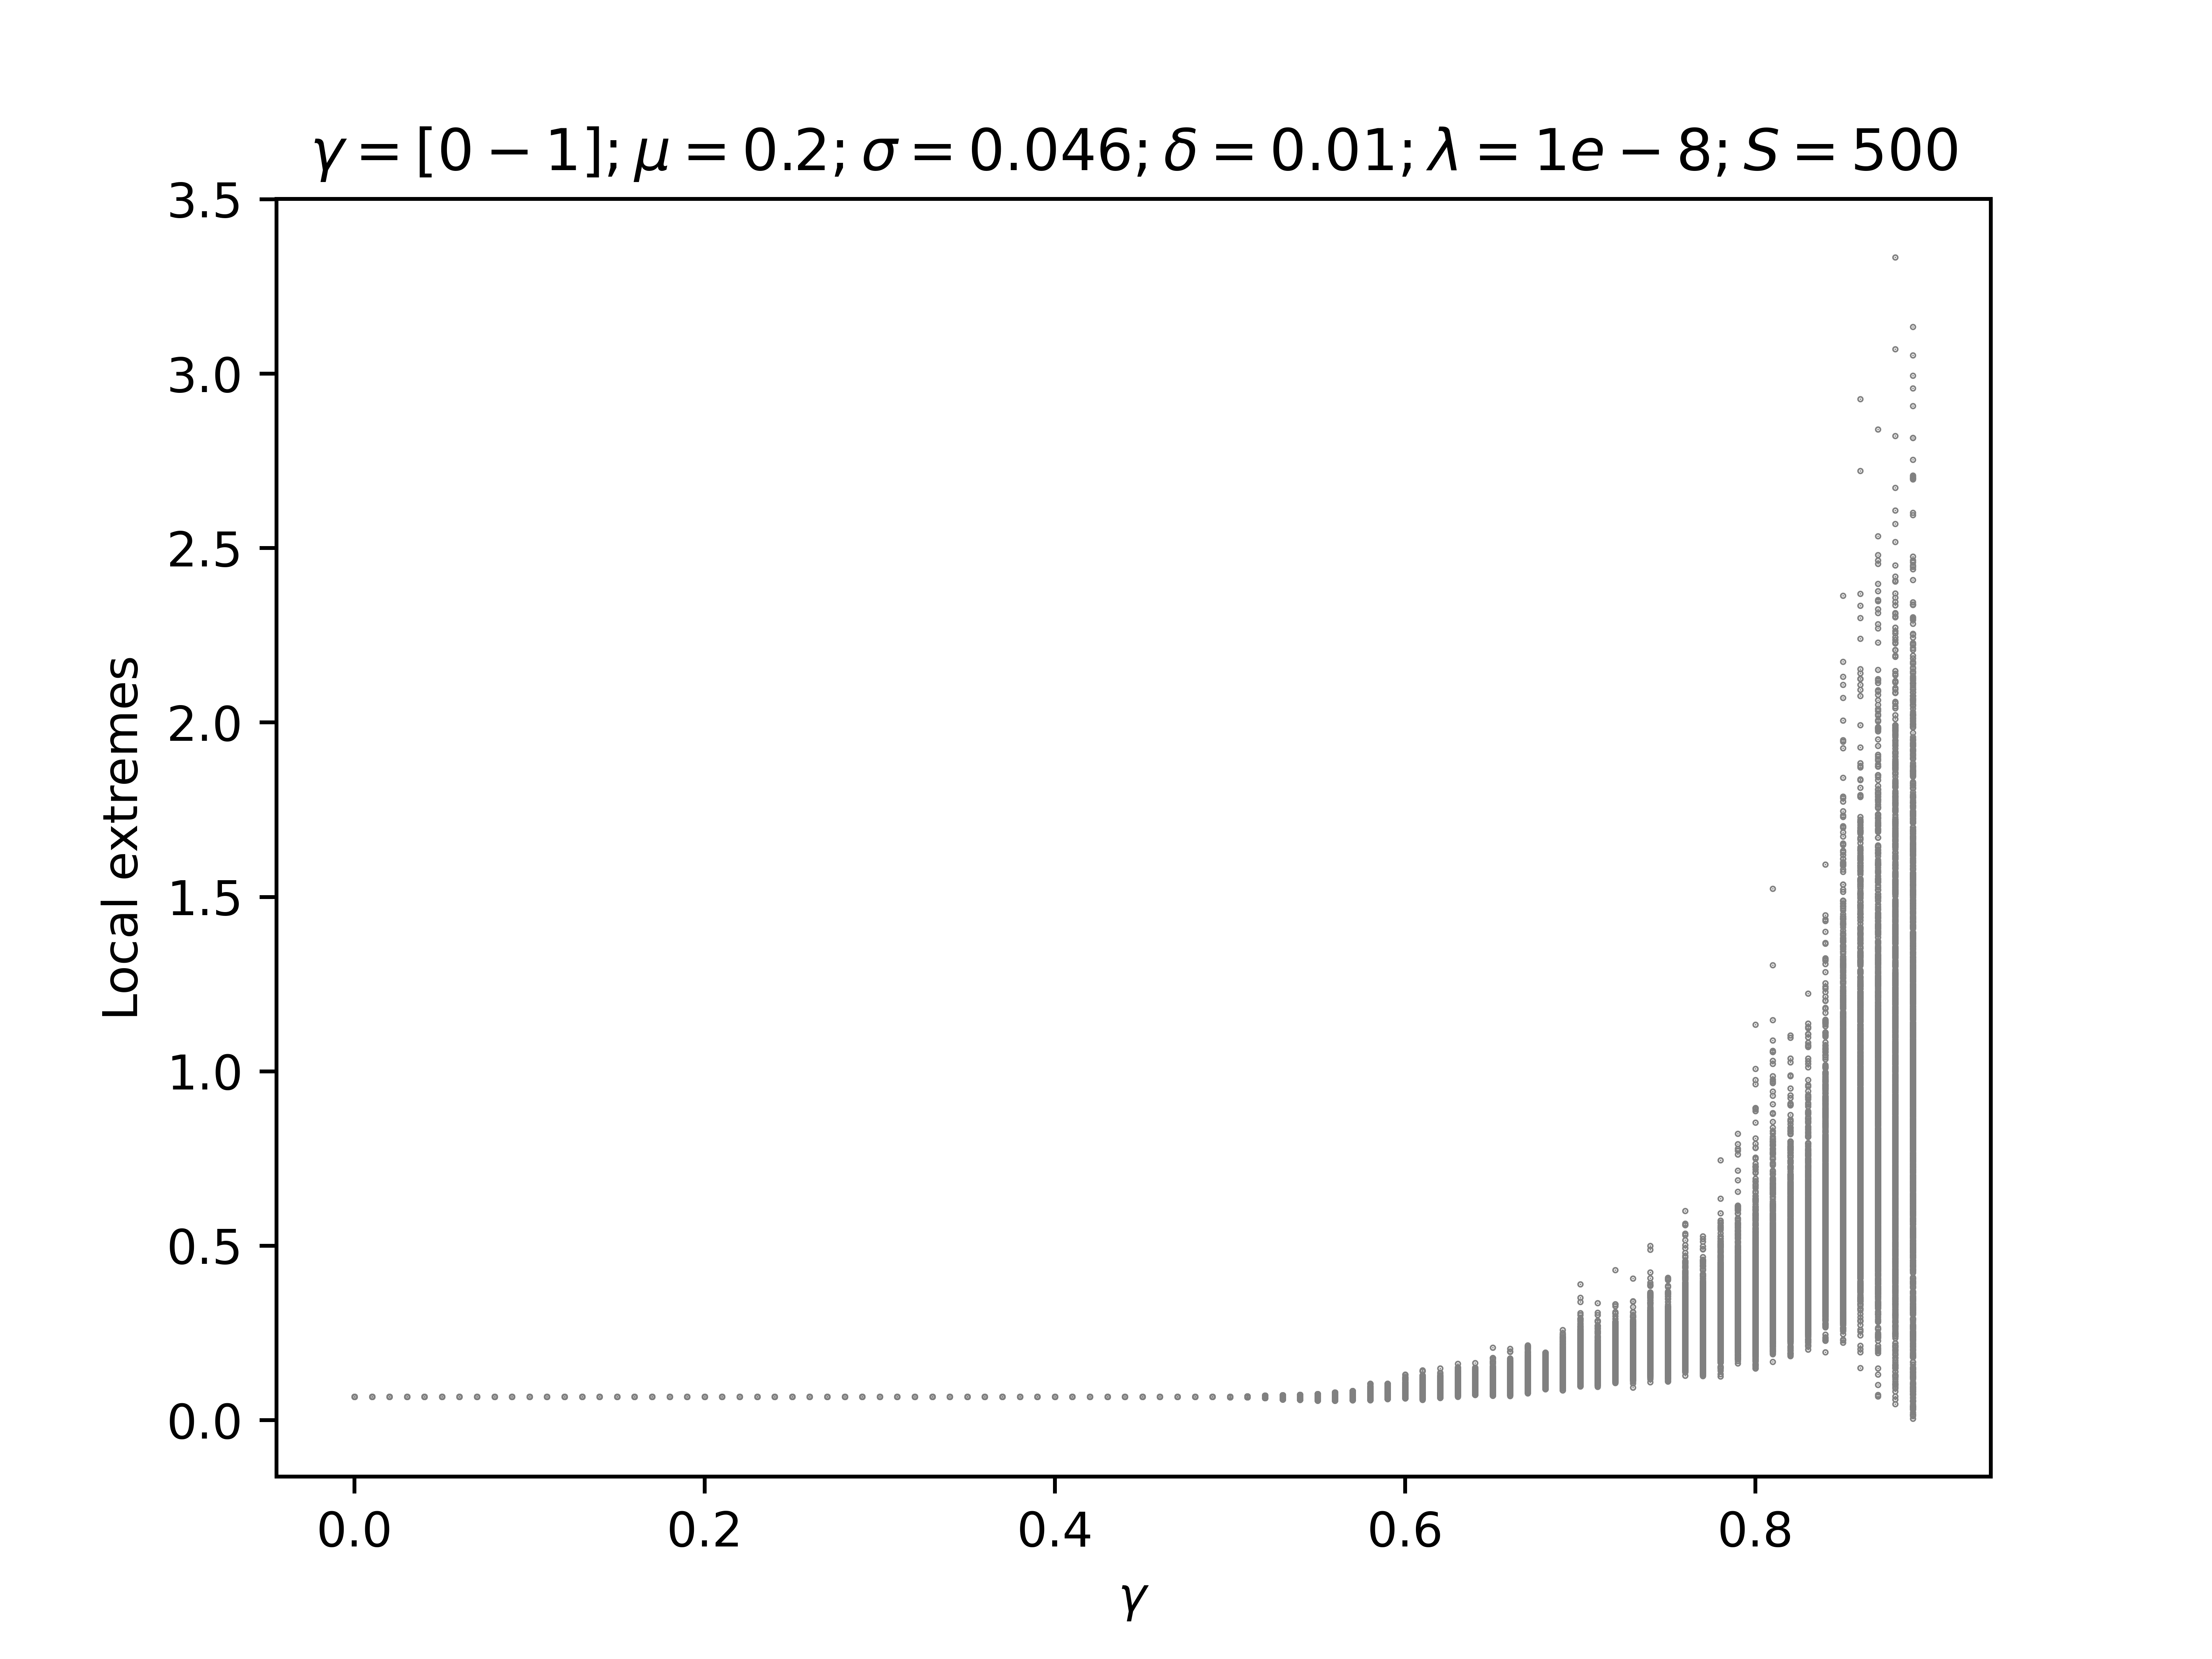
\includegraphics[width=\linewidth]{Bifurcation/BifurcationM1.png}
    \caption{Abundance of the most abundant species as a function of $\gamma$.}
\end{figure}
\clearpage

\subsubsection{Varying $\delta$ from 0.001 to 0.022}

\begin{figure}[H]
    \centering
    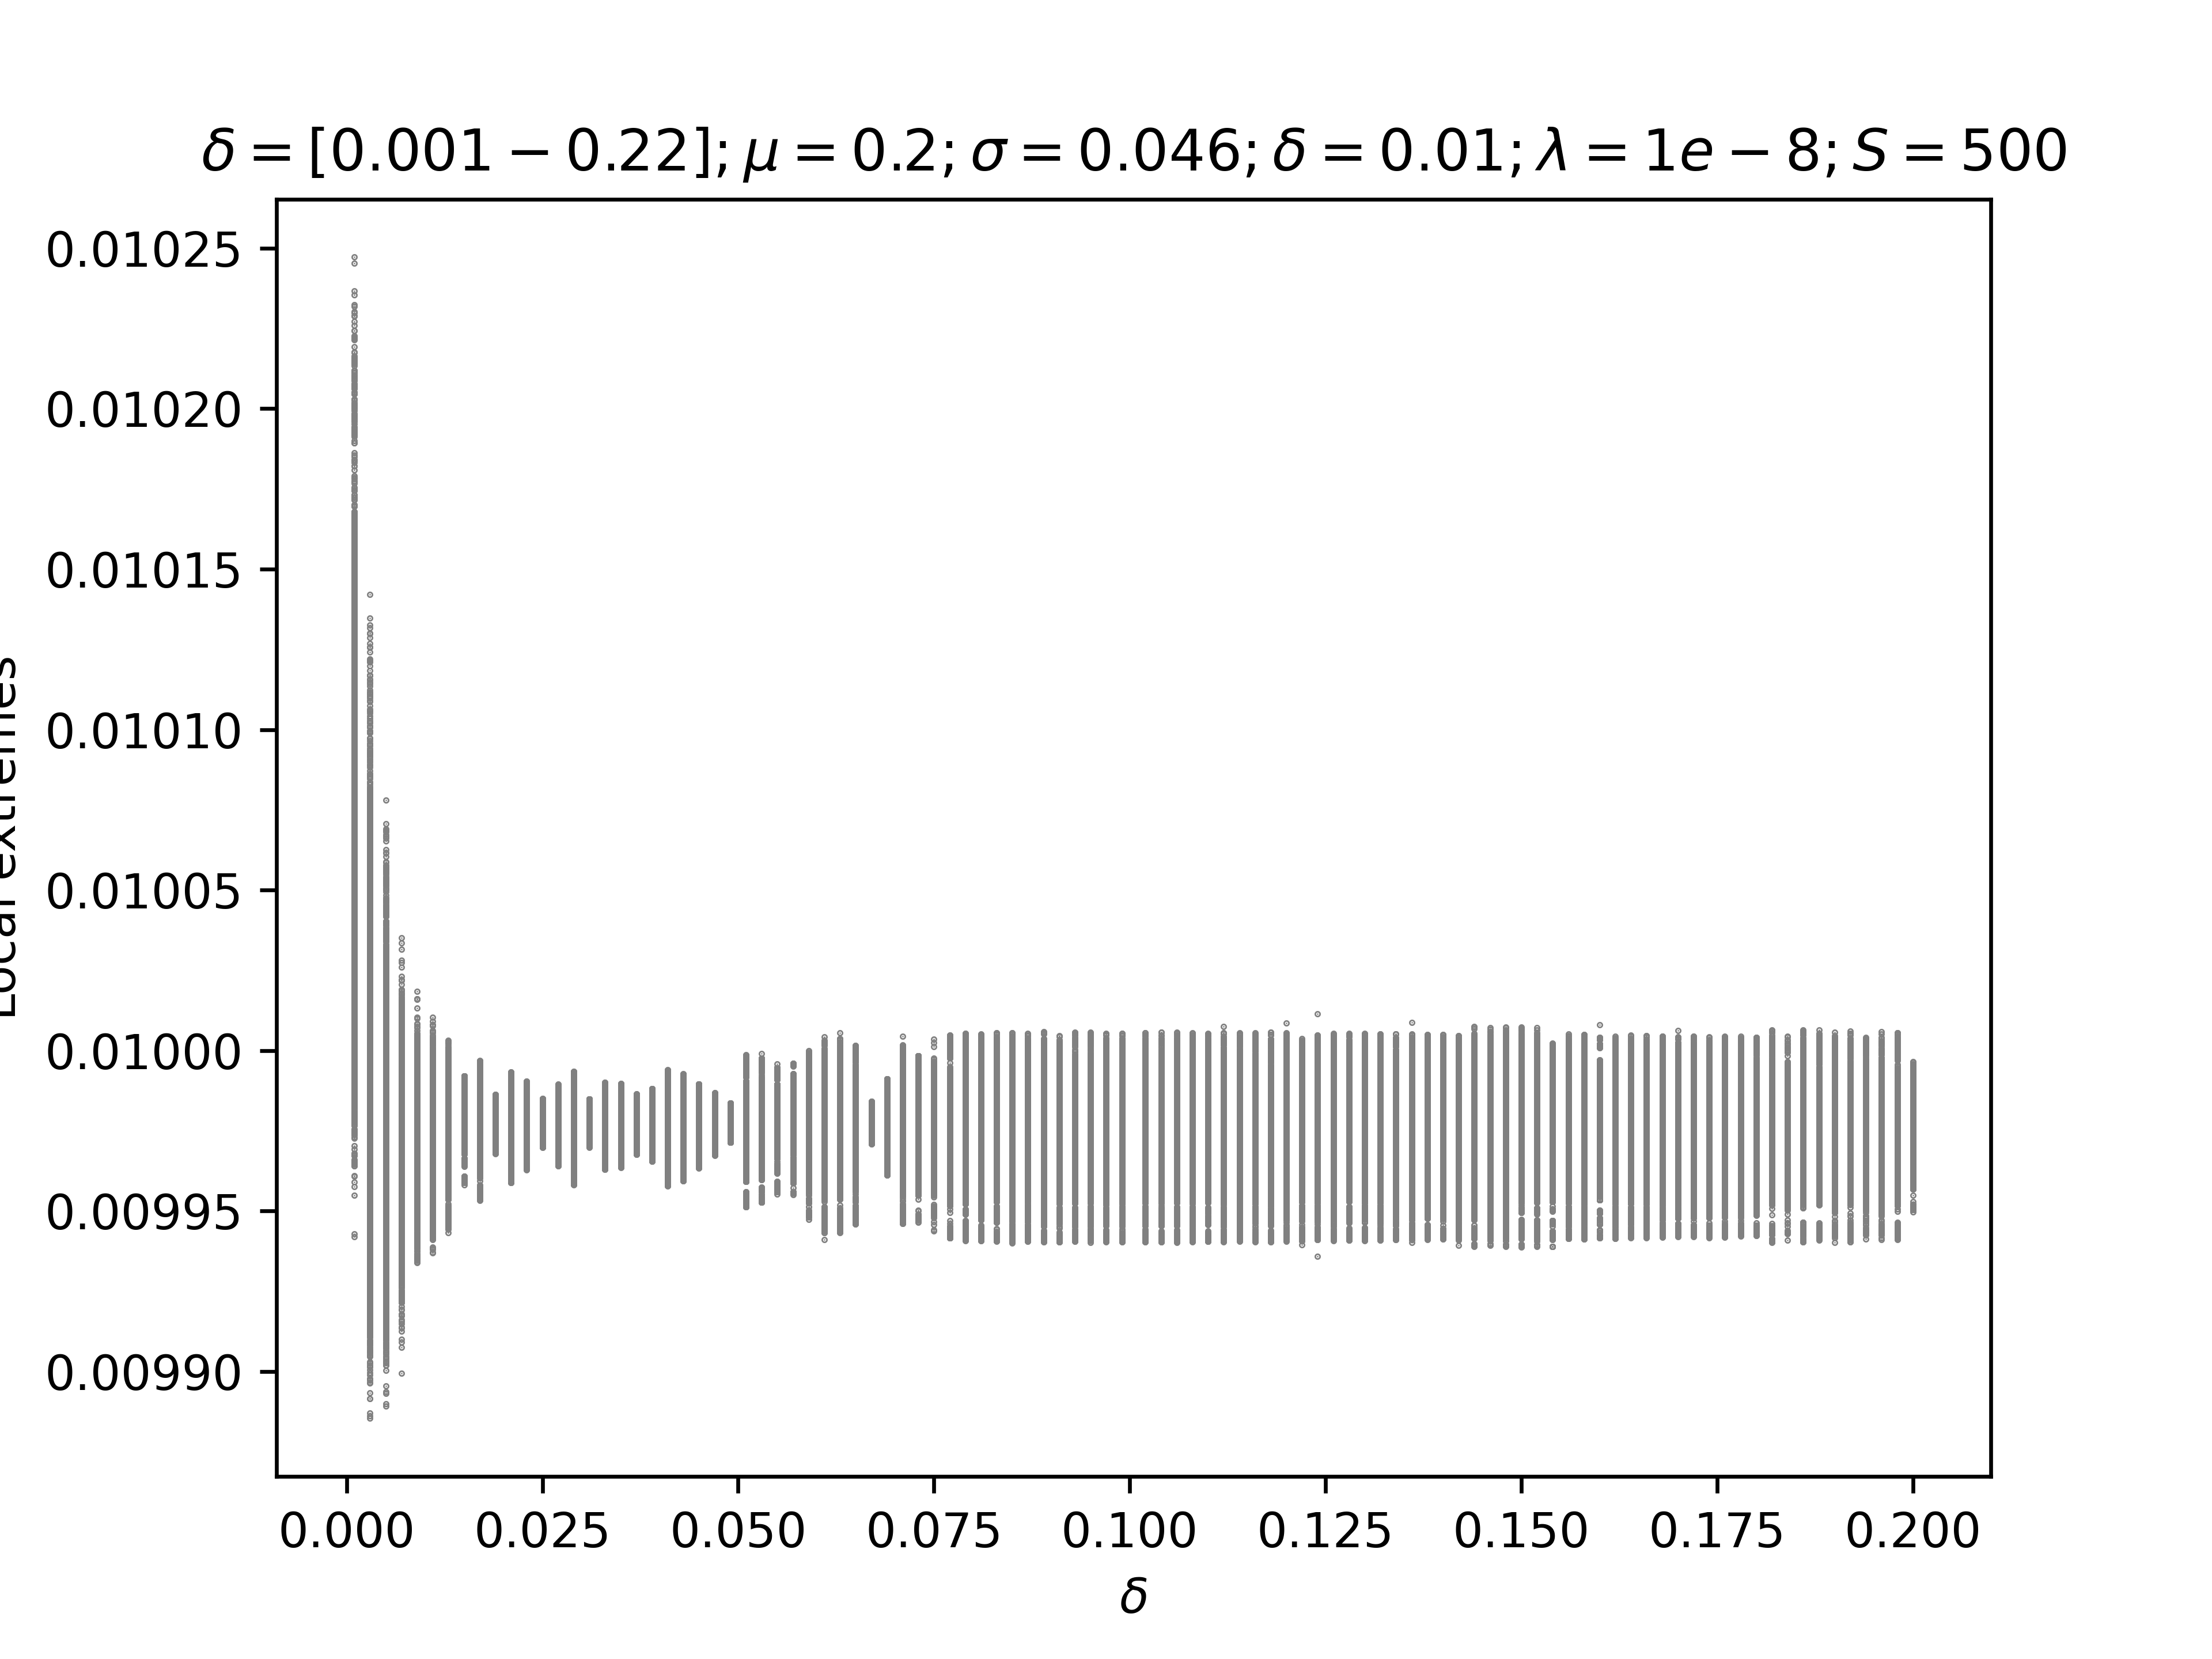
\includegraphics[width=\linewidth]{Bifurcation/BifurcationMeanDelta.png}
    \caption{Mean abundance of all species as a function of $\delta$.}
\end{figure}

\begin{figure}[H]
    \centering
    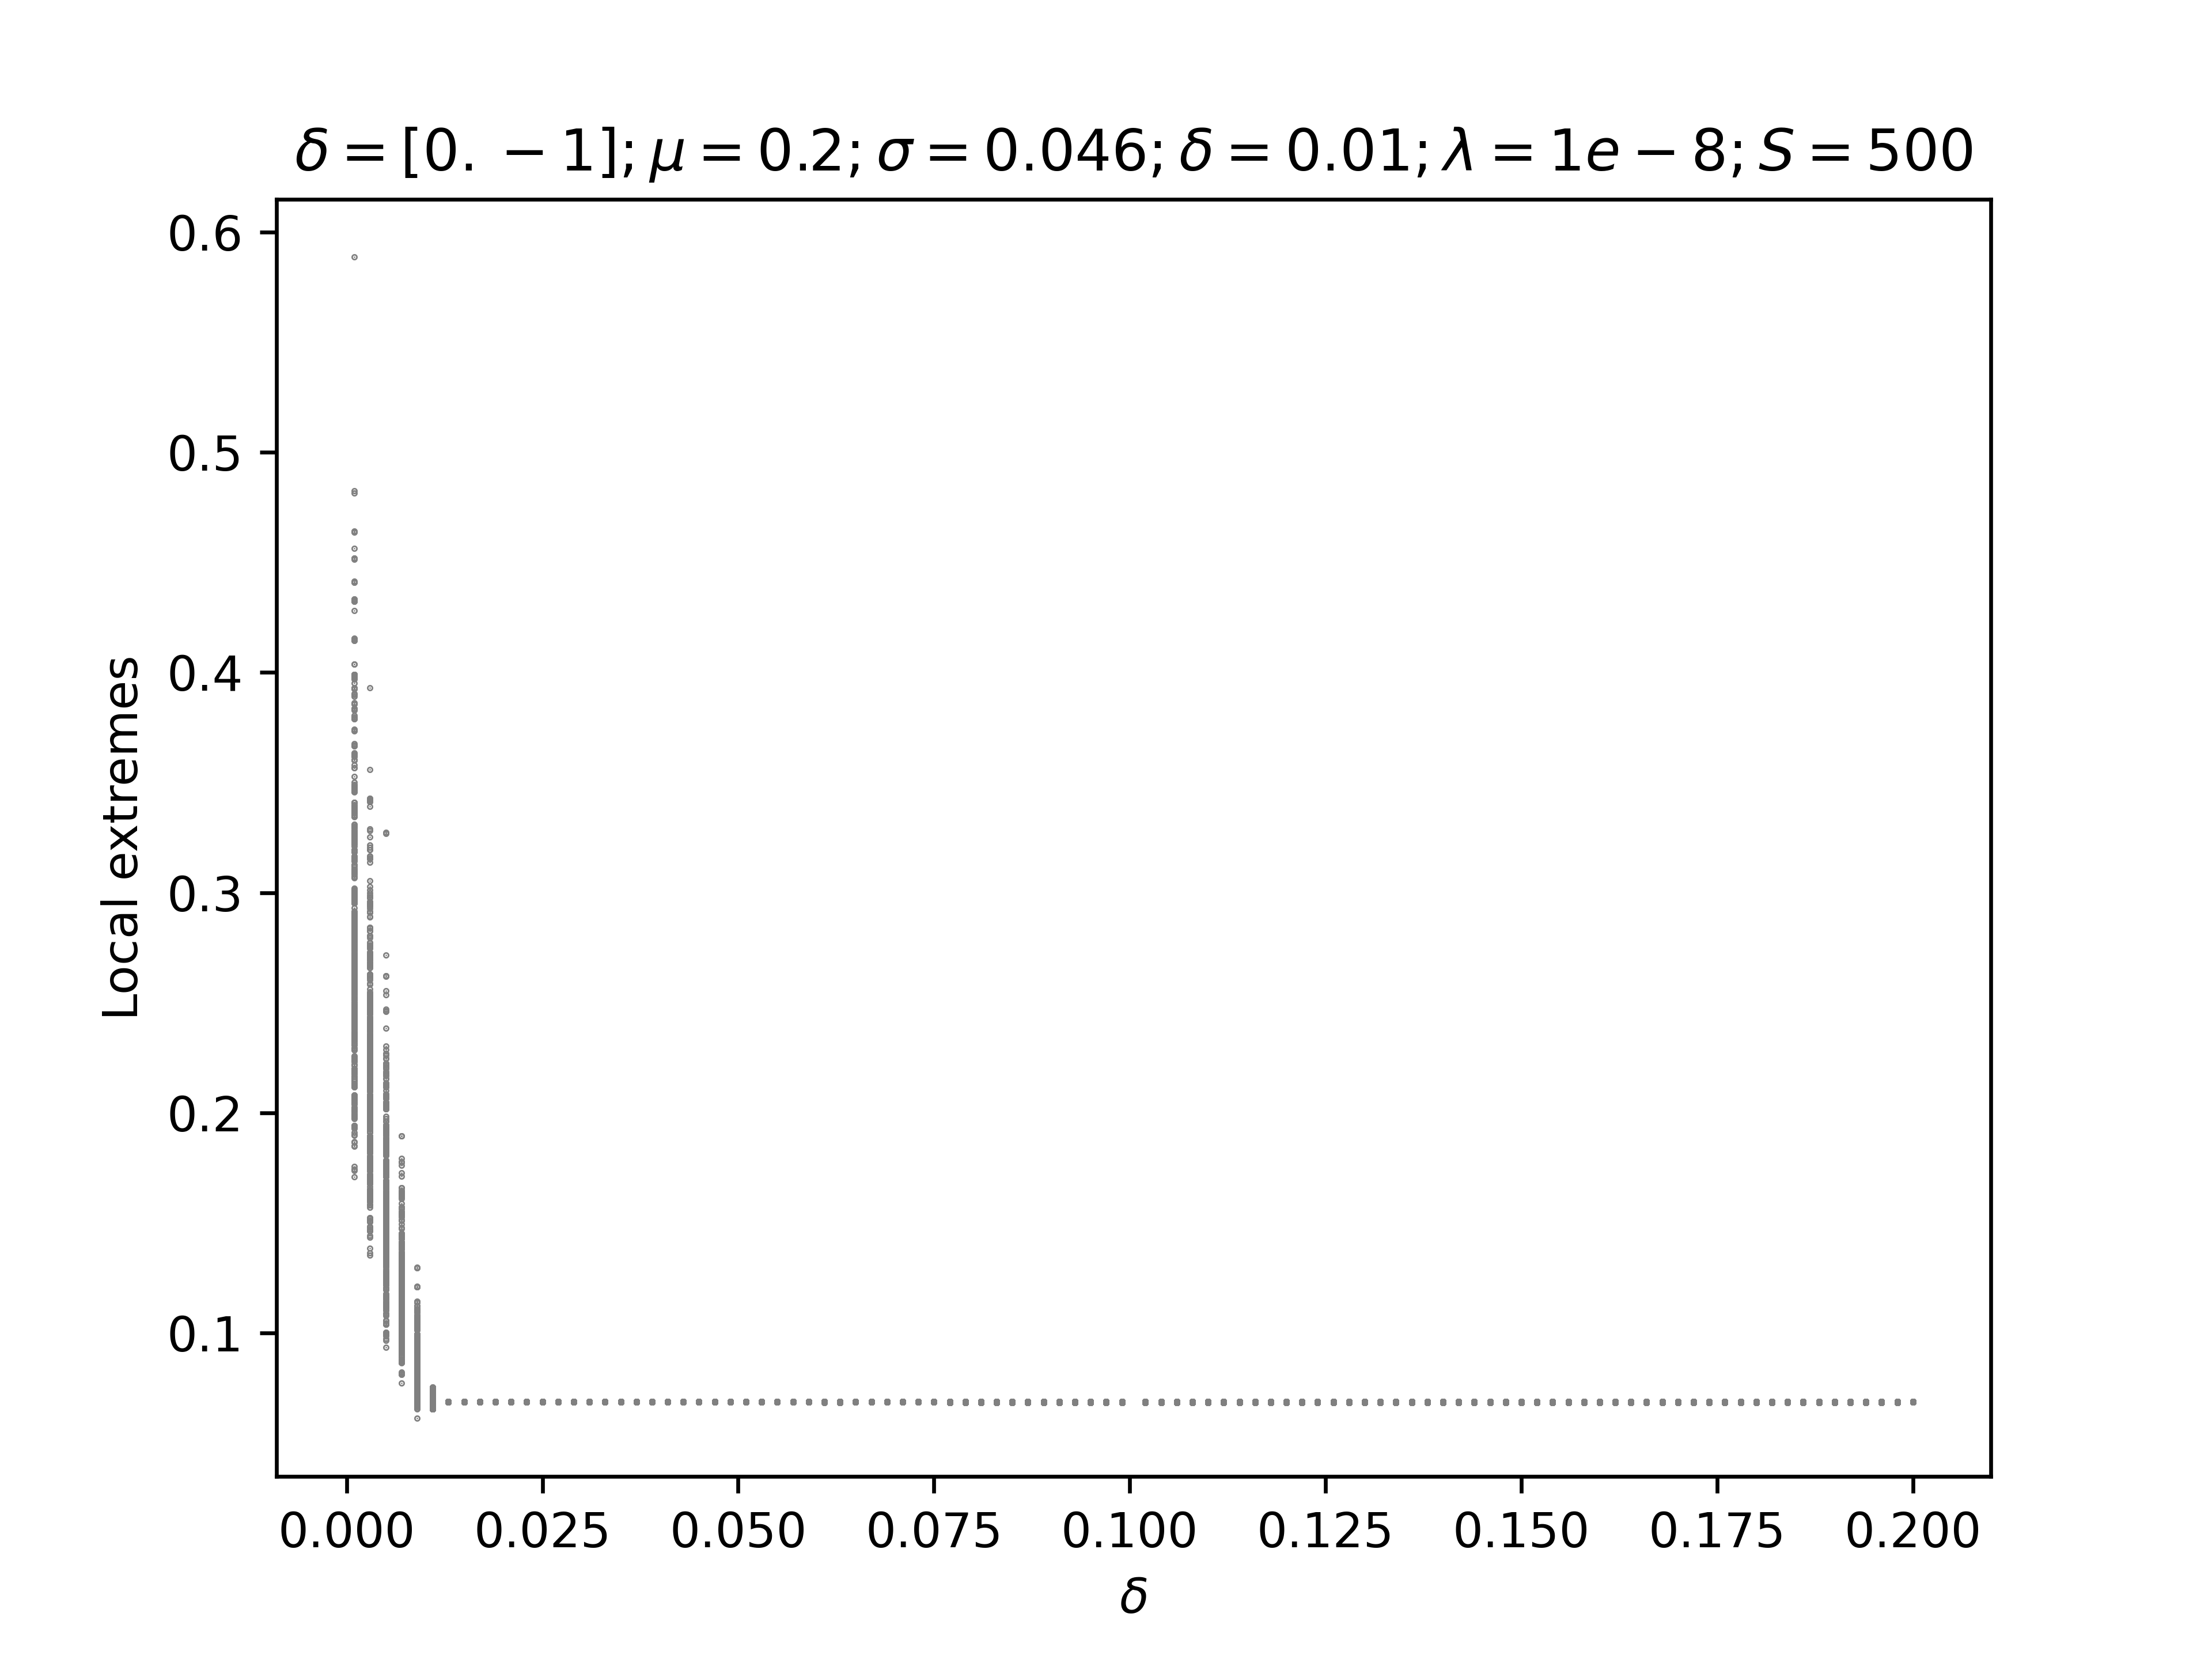
\includegraphics[width=\linewidth]{Bifurcation/BifurcationM1Delta.png}
    \caption{Abundance of the most abundant species as a function of $\delta$.}
\end{figure}
\clearpage
\end{document}